\chapter{Badanie skuteczności metod}
Wszystkie testy zostały przeprowadzone 10 razy z tymi samymi parametrami lecz za każdym razem z nowo wylosowanymi dokumentami, poddanymi wcześniej fazom przetwarzania, lematyzacji, wektoryzacji, a następnie klasyfikacji. Wyniki z iteracji tych samych testów zostały uśrednione i przedstawione na wykresach. 

\section{Korpus porównawczy}
Do celów porównawczych wykorzystano dodatkowo korpus o nazwie \textit{Wiki train - 34 categories}, dostępny w repozytorium Clarin \cite{11321/222}. Składa się on z 6800 dokumentów podzielonych na 34 klasy. Został on poddany tym samym procesom przetwarzania, co zebrany korpus z artykułami. Poszczególne kroki przetwarzania zostały pokazane na rysunku \ref{fig:process-flow}.

\begin{figure}[ht!]
	\centering
	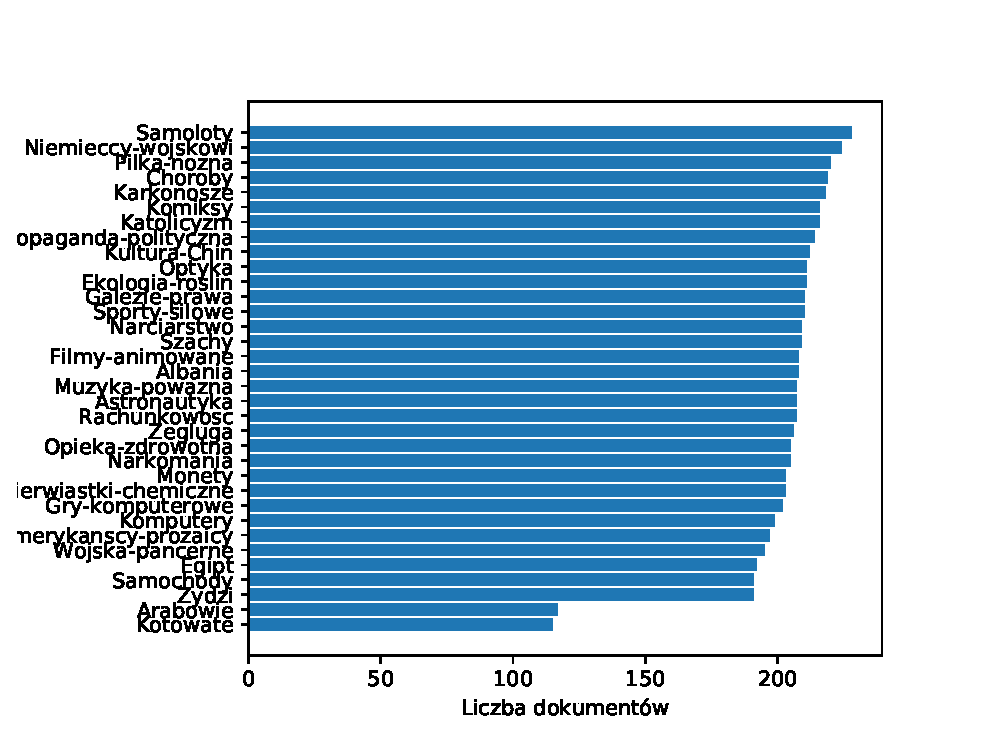
\includegraphics[width=0.8\linewidth]{img/count-files-wikipedia}
	\caption{Porównanie ilości dokumentów dla każdej klasy dla korpusu Wikipedii}
\end{figure}

\newpage
\section{Badane parametry}

Do określenia jakości wykorzystano cztery różne powszechnie stosowane parametry miar jakościowych \cite{walkowiak2018} \cite{maciej-baj}. Dodatkowo zmierzony został czas pracy każdego z klasyfikatorów nad różnymi etapami pracy.



\begin{itemize}
 \setlength\itemsep{2em}
\item \textbf{czułość} (ang. recall) - jest liczbą poprawnych pozytywnych wyników podzieloną przez liczbę wszystkich odpowiednich próbek (wszystkie próbki, które powinny zostać zidentyfikowane jako pozytywne). \cite{skl-reference} Czułość określa się wzorem:

\begin{equation}
\label{recallEq}
R = \frac{T_{p}}{T_{p} + F_{n}}
\end{equation}
Gdzie:
\begin{itemize}
\item $T_{p}$ - oznacza liczbę poprawnie rozpoznanych dokumentów
\item $F_{n}$ - oznacza liczbę niepoprawnie nierozpoznanych dokumentów
\end{itemize}

\item \textbf{precyzja} (ang. precision) - jest liczbą poprawnych pozytywnych wyników podzieloną przez liczbę wszystkich pozytywnych wyników zwróconych przez klasyfikator. \cite{skl-reference} Precyzję określa się wzorem:

\begin{equation}
\label{precisionEq}
P = \frac{T_{p}}{T_{p} + F_{p}}
\end{equation}
Gdzie:
\begin{itemize}
\item $T_{p}$ - oznacza liczbę poprawnie rozpoznanych dokumentów
\item $F_{p}$ - oznacza liczbę niepoprawnie rozpoznanych dokumentów
\end{itemize}

\item \textbf{miara f1} (ang. f1-score) - w statystycznej analizie klasyfikacji jest to miara dokładności testu. Uwzględnia ona dwa wcześniejsze parametry: precyzję oraz czułość. Jest średnią harmoniczną, gdzie wynik F1 osiąga najwyższą wartość 1 (doskonała precyzja i czułość), a najgorszy - 0. \cite{miary-jakosci}

\begin{equation}
F1 = 2*\frac{P * R}{P+R}
\end{equation}

Gdzie:
\begin{itemize}
\item $P$ - oznacza precyzję opisywaną we wzorze \ref{precisionEq}
\item $R$ - oznacza czułość opisywaną we wzorze \ref{recallEq}
\end{itemize}

\item \textbf{dokładność} (ang. accuracy) - stosunek między poprawnie sklasyfikowanymi dokumentami do wszystkich dokumentów. \cite{skl-reference}

\begin{equation}
A = \frac{T_{p} + T_{n}}{T_{p} + T_{n} + F_{p} + F_{n}}
\end{equation}

Gdzie:
\begin{itemize}
\item $T_{p}$ - oznacza liczbę poprawnie rozpoznanych dokumentów
\item $T_{n}$ - oznacza liczbę poprawnie nierozpoznanych dokumentów
\item $F_{p}$ - oznacza liczbę niepoprawnie rozpoznanych dokumentów
\item $F_{n}$ - oznacza liczbę niepoprawnie nierozpoznanych dokumentów
\end{itemize}
\end{itemize}


Dodatkowo w testach uwzględniono inne miary niż jakościowe, a mianowicie:
\begin{itemize}
\item \textbf{czas nauki klasyfikatora} - czas wyrażony w sekundach, potrzebny systemowi na naukę danego klasyfikatora danymi wejściowymi. Ściślej mówiąc, jest to czas potrzebny na wykonanie się metod; był odpowiedzialny za nauczenie modelu dla każdego użytego klasyfikatora. 

\item \textbf{czas klasyfikacji} - czas wyrażony w sekundach, potrzebny systemowi na klasyfikację zbioru dokumentów. 

\item \textbf{całkowity czas pracy} - czas wyrażony w sekundach, jest to suma czasu potrzebnego na naukę oraz klasyfikację zbioru dokumentów.
\end{itemize}

\section{Wyniki testów}

Całość badanego korpusu z artykułami składała się z 2600 artykułów, podzielonych na 7 klas, po 380 dokumentów dla każdej kategorii. Szczegółowe informacje dotyczące wykorzystanych korpusów przedstawiono w tabeli \ref{fig:korpus-compare}. Z tego zbioru część artykułów przeznaczono do trenowania oraz część do testowania. W przypadku krzywej nauczania, wszystkie artykuły brały udział w teście. Ilość danych testowych była uzależniona od liczby danych uczących i była liczbą, która pozostała po odjęciu liczby dokumentów niebiorących udziału w fazie nauczania. Badania rozpoczęto od próby dopasowania optymalnych parametrów dla danego zbioru danych. Z obu pełnych korpusów zostały wyznaczone dwa dodatkowe, zawierające jedynie formy podstawowe rzeczowników, sklasyfikowane przy pomocy analizatora WCRTF2 podczas przetwarzania wstępnego. Taki korpus został podpisany hasłem \textit{rzeczowniki}.

\begin{table}[ht!]
\centering
\caption{Porównanie badanych korpusów danych}
\label{fig:korpus-compare}
\begin{tabular}{|l|l|l|l|l|}
\hline
nazwa korpusu & l. dokumentów & l. klas & l. dokumentów na klasę & rozmiar na dysku \\ \hline
Wikipedia     & $\sim$6800        & 34         & $\sim$200 & 34MB               \\ \hline
Artykuły      & $\sim$2600        & 7          & $\sim$380  & 12MB              \\ \hline
Wikipedia (rzeczowniki)     & $\sim$6800        & 34         & $\sim$200 & 28MB               \\ \hline
Artykuły (rzeczowniki)     & $\sim$2600        & 7          & $\sim$380 & 8.6MB               \\ \hline
\end{tabular}
\end{table}

\subsection{Bag-Of-Words}

W modelu \textit{Bag-Of-Words} w każdym teście została domyślnie użyta normalizacja \textit{tf-idf} z listą słów nierelewantnych. Zmieniany był parametr n-gram oraz rodzaj zawartości n-gramów. Przetestowano dwa różne scenariusze:
\begin{itemize}
\item Scenariusz 1: analiza słów n-gramowych dla wartości parametru \textit{n-gram}: 1, 2, 3
\item Scenariusz 2: analiza znaków n-gramowych dla wartości parametru \textit{n-gram}: 5, 6, 7
\end{itemize}
Testy zostały przeprowadzone z wykorzystaniem trzech klasyfikatorów (NaiveBayes, SVM, drzewo decyzyjne) a wyniki zostały uśrednione w celu zwiększenia czytelność wykresów oraz opisane pod wspólną nazwą \textit{BoW} na wykresach. Scenariusze zostały przetestowane dla obydwu wykorzystywanych w pracy korpusów.

W przypadku analizy znaków, lista \textit{stop words} nie była wykorzystywana i żadne słowa nie zostały odrzucone. 

\begin{figure}[ht!]
	\centering
	\subfloat[Artykuły]{{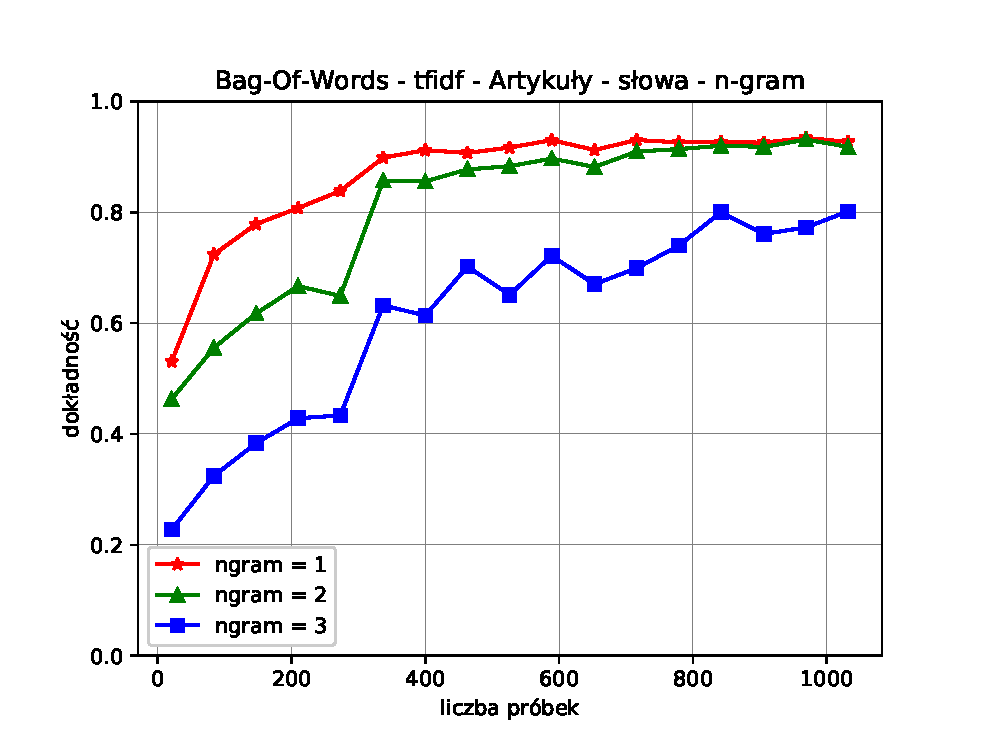
\includegraphics[width=0.45\linewidth]{img/bag-of-words-tfidf-articles-words-n-gram}}}
    \qquad
    \subfloat[Wikipedia]{{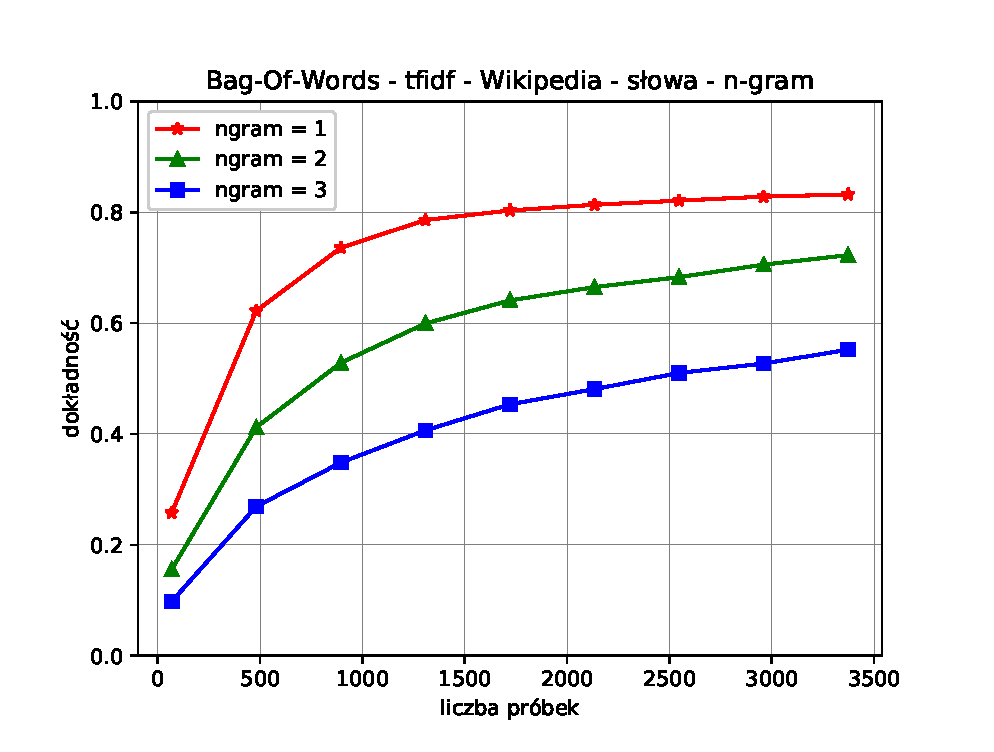
\includegraphics[width=0.45\linewidth]{img/bag-of-words-tfidf-wikipedia-words-n-gram}}}
	\caption{Porównanie dokładności klasyfikacji \textit{Bag-Of-Word} dla n-gramów składających się ze słów - Scenariusz 1}
    \label{fig:bow-ngram-compare-word}
\end{figure}

W pierwszym testowanym scenariuszu \ref{fig:bow-ngram-compare-word} dokładność klasyfikacji była niższa dla większych wartości \textit{n-gram}, co jest zgodne z intuicją. Większa ilość słów wchodzących w skład n-gramu, w przypadku niewielkiej ilości danych, zwraca niższe rezultaty; jest to spowodowane większą trudnością odnalezienia i dopasowania takiego samego n-gramu. Wykres \ref{fig:bow-ngram-compare-word} pokazuje, że bigramy oraz unigramy uzyskały ostatecznie zbliżone wyniki. Wynika to prawdopodobnie z faktu, iż liczba klas była mniejsza, przez co pojawiało się zdecydowanie mniej unikalnych słów w korpusie. 

\begin{figure}[ht!]
	\centering
	\subfloat[Artykuły]{{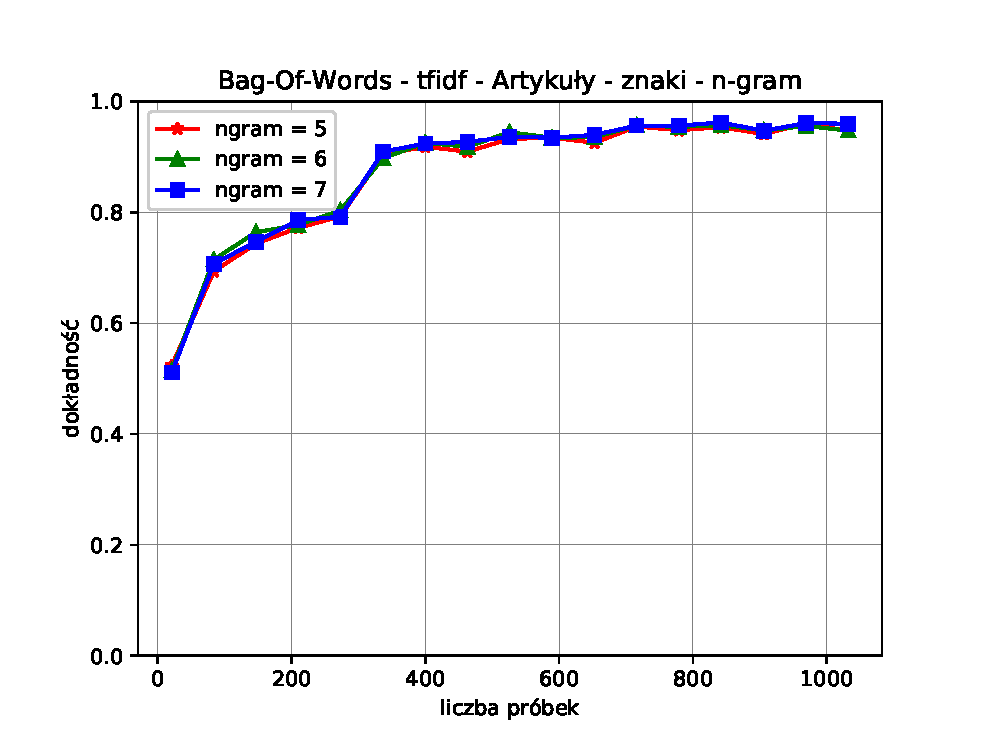
\includegraphics[width=0.45\linewidth]{img/bag-of-words-tfidf-articles-char-n-gram}}}
    \qquad
    \subfloat[Wikipedia]{{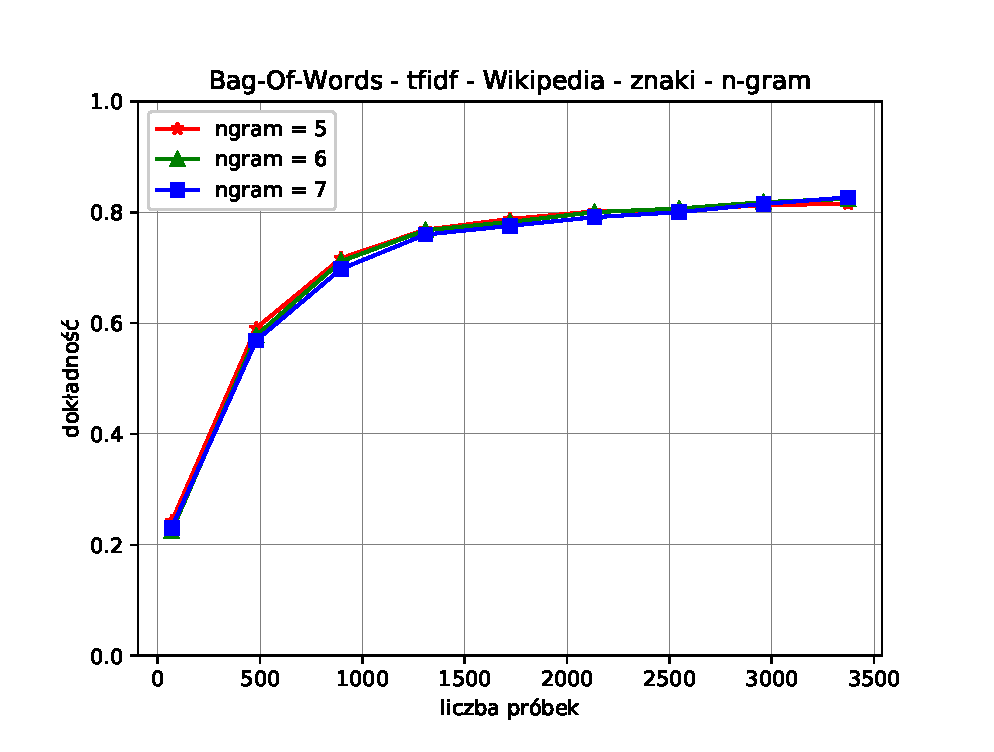
\includegraphics[width=0.45\linewidth]{img/bag-of-words-tfidf-wikipedia-char-n-gram}}}
	\caption{Porównanie dokładności klasyfikacji \textit{Bag-Of-Word} dla n-gramów składających się ze znaków - Scenariusz 2}
    \label{fig:bow-ngram-compare-char}
\end{figure}

W drugim testowanym scenariuszu nie stwierdzono większych różnic pomiędzy użytymi wartościami parametrów. Wyniki końcowe wykazały, że użycie n-gramów składających się ze słów, w tym przypadku zwraca lepsze wyniki niż użycie n-gramów składających się ze znaków. Wyniki końcowe z najlepszymi uzyskanymi wartościami dokładności i odpowiadającym im parametrom przedstawiono w tabeli \ref{tab:bow-scenario-results}.

\begin{table}[]
\centering
\caption{Najlepsze wyniki testów \textit{Bag-Of-Words} dla różnych wartości n-gram i rodzaju analizowanych n-gramów}
\label{tab:bow-scenario-results}
\begin{tabular}{|l|c|c|c|}
\hline
scenariusz & nazwa korpusu                         & n-gram & dokładność \\ \hline
Scenariusz 1                     & Artykuły                       & 1 (słowa)     & 0.92                            \\ \hline
Scenariusz 1                     & Wikipedia & 1 (słowa)     & 0.82                            \\ \hline
Scenariusz 2                     & Artykuły  & 7 (znaki)      & 0.96                            \\ \hline
Scenariusz 2                     & Wikipedia                      & 5 (znaki)      & 0.82                            \\ \hline
\end{tabular}
\end{table}


Użycie modelu \textit{n-gramowego} dla znaków mogłoby zwracać lepsze rezultaty w przypadku dużej liczby słów, których analizatory morfologiczne nie były w stanie poprawnie rozpoznać i sprowadzić do ich form podstawowych. Przykładem mogłaby być sytuacja, kiedy w tekście znajduje się duża liczba literówek - uniemożliwiłoby to poprawne porównanie dwóch takich samych słów jednak napisanych z błędami.

\subsection{fastText}
Biblioteka \textit{fastText} według założeń przyjmuje zbiory dokumentów, bez żadnych modyfikacji. \cite{joulin2016fasttext} W pracy podjęto próbę optymalizacji tej metody, mającą na celu zmniejszenie czasu pracy bez wpływu na jakość wyników. W celu ograniczenia zbioru dokumentów wejściowych dla \textit{fastText}, zostały one poddane takiemu samemu procesowi jak w metodzie \textit{BoW}; proces ten został przedstawiony na rysunku \ref{fig:process-flow}. W celu wyboru optymalnych parametrów dla zmodyfikowanych korpusów wejściowych, przetestowano zmianę każdego z parametrów przy pozostawieniu domyślnych parametrów dla pozostałych wartości. Za najlepszą wartość parametru przyjmowano tą, przy użyciu której ostatecznie zwracane były najwyższe wyniki dla miary dokładności. Rezultaty przy użyciu zmienionych parametrów zostały zaznaczone na wykresach jako \textit{fastText (zmodyfikowany)}\footnote{W dalszej części pracy \textit{fastText (zmodyfikowany)} jest również zamiennie określany jako \textit{fastText}.}. Wyniki zostały uśrednione po 10 przebiegach dla każdego testu.


\subsubsection{Zmiana parametru \textit{ngram}}


\begin{figure}[ht!]
	\centering    
    \subfloat[Artykuły]{{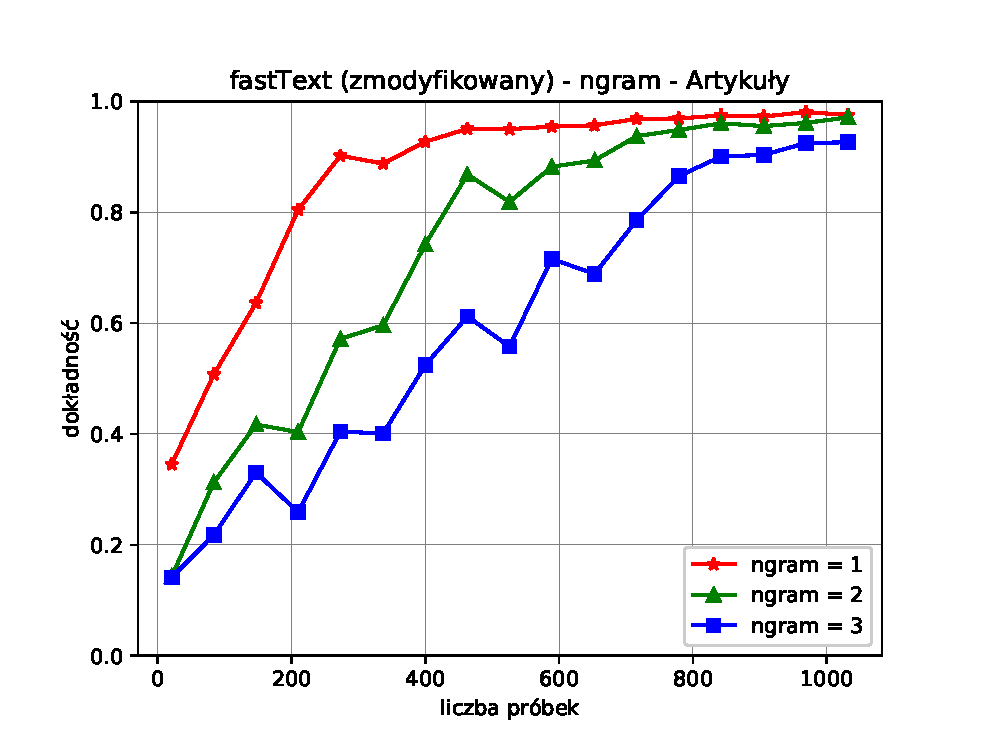
\includegraphics[width=0.45\linewidth]{img/fasttext-ngram-articles}}}
    \qquad
    \subfloat[Artykuły (rzeczowniki)]{{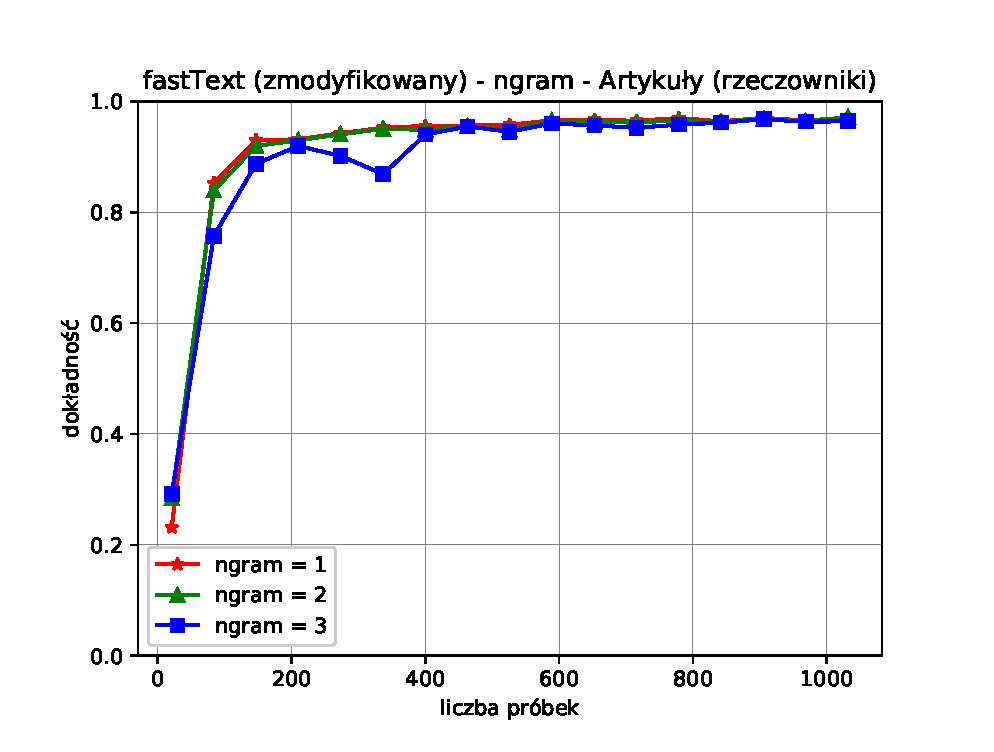
\includegraphics[width=0.45\linewidth]{img/fasttext-ngram-articles-nouns}}}
    
    \subfloat[Wikipedia]{{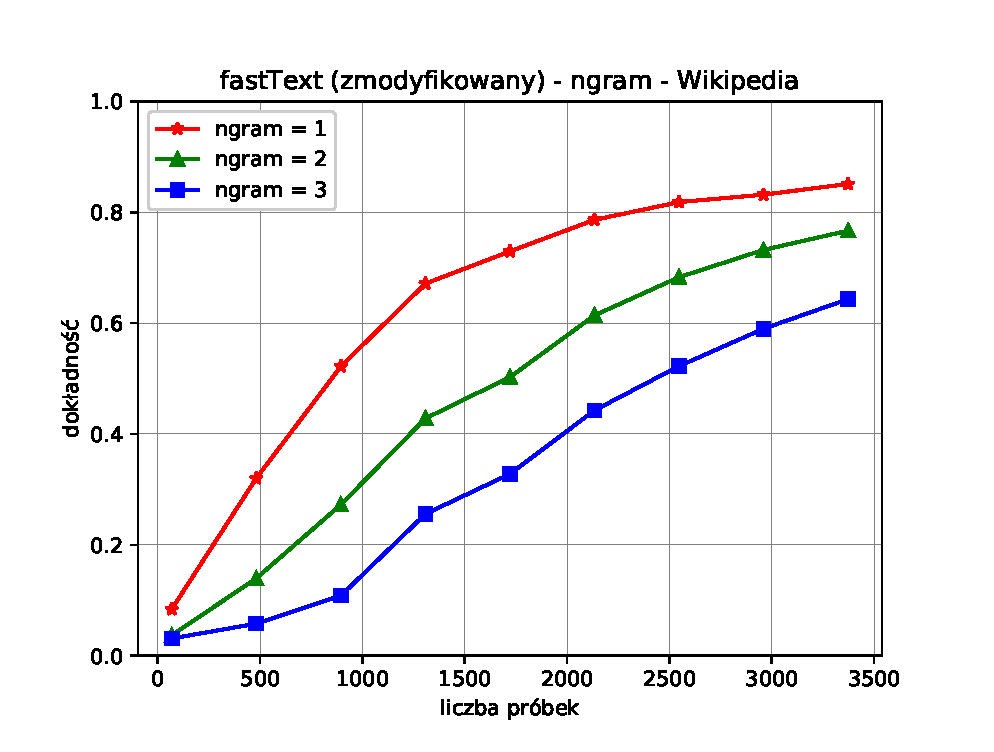
\includegraphics[width=0.45\linewidth]{img/fasttext-ngram-wikipedia}}}
    \qquad
    \subfloat[Wikipedia (rzeczowniki)]{{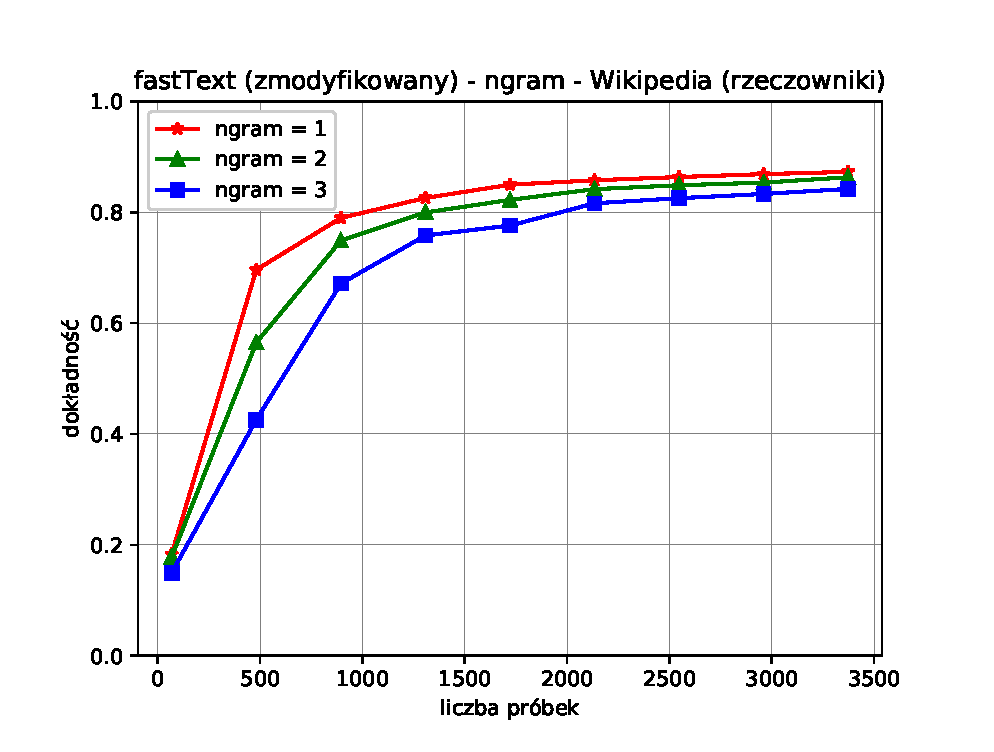
\includegraphics[width=0.45\linewidth]{img/fasttext-ngram-wikipedia-nouns}}}
    
	\caption{Porównanie wyników zmiany parametru \textit{n-gram}}
    \label{fig:fasttext-ngram}
\end{figure}


Parametr \textit{ngram} określa maksymalną długość na jaką zostanie podzielony zbiór wyrazów.
Wszystkie trzy instancje w początkowej fazie osiągnęły podobny wynik dokładności, kolejne iteracje wskazały że instancja z parametrem \textit{ngram=1} uczyła się najszybciej i to ona ostatecznie osiągnęła też najlepsze wyniki, dla wszystkich czterech przypadków. Jest to skutek odwrotny do oczekiwanego, w żadnym momencie \textit{fastText} z użyciem bigramów nie osiągnął lepszego wyniku niż unigramy \cite{joulin2016bag}. Powodem takich rezultatów jest prawdopodobnie fakt, iż w przypadku korpusu z artykułami bardziej informacyjne były unigramy niż formy zawierające więcej n-gramów. Wyniki zostały przedstawione na rysunku \ref{fig:fasttext-ngram}.

\subsubsection{Zmiana parametru \textit{min\_count}}
Parametr \textit{min\_count} odrzuca wyrazy, które występują częściej niż zadana wartość, wyniki zmiany parametru zaprezentowano na rysunku \ref{fig:fasttext-mincount}.



\begin{figure}[ht!]
	\centering    
    \subfloat[Artykuły]{{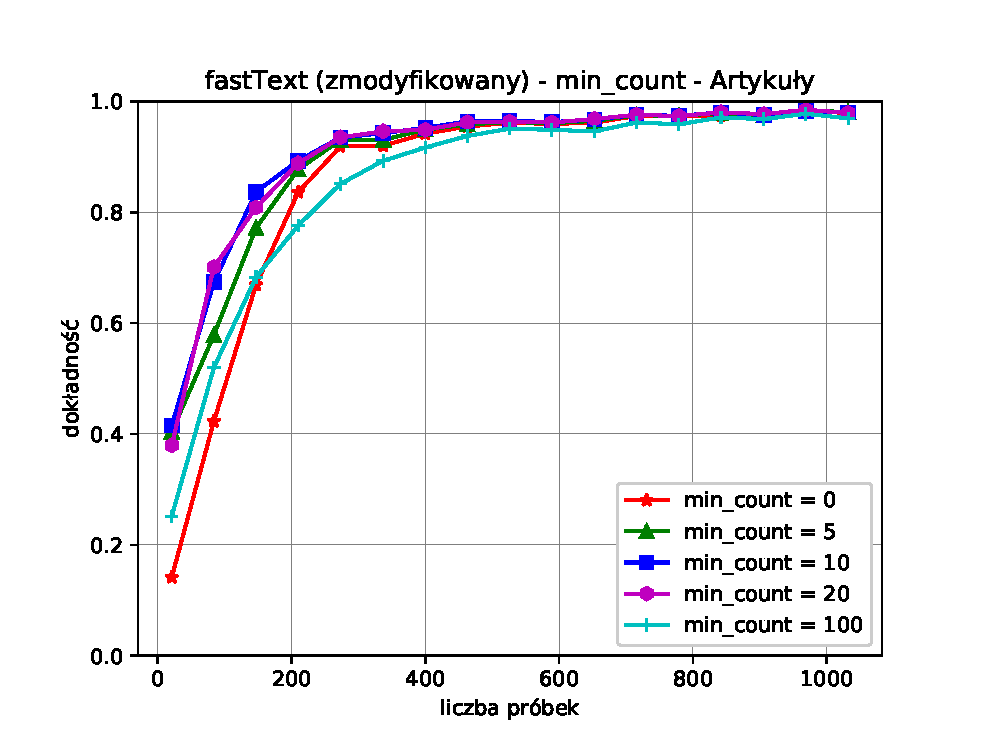
\includegraphics[width=0.45\linewidth]{img/fasttext-min_count-articles}}}
    \qquad
    \subfloat[Artykuły (rzeczowniki)]{{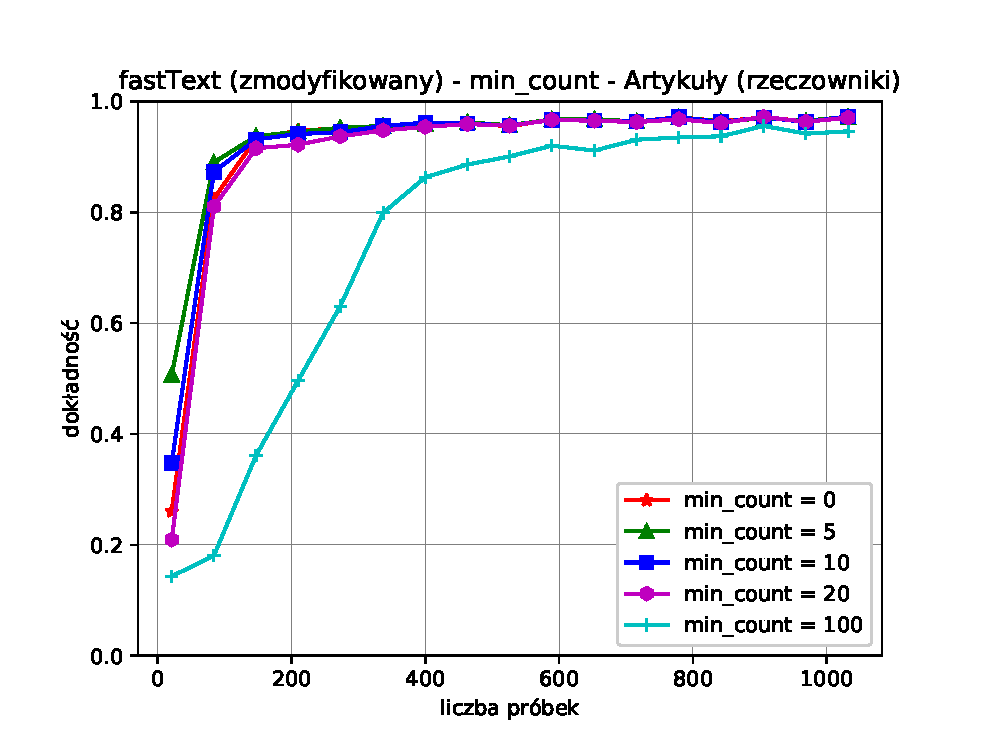
\includegraphics[width=0.45\linewidth]{img/fasttext-min_count-articles-nouns}}}
    
    \subfloat[Wikipedia]{{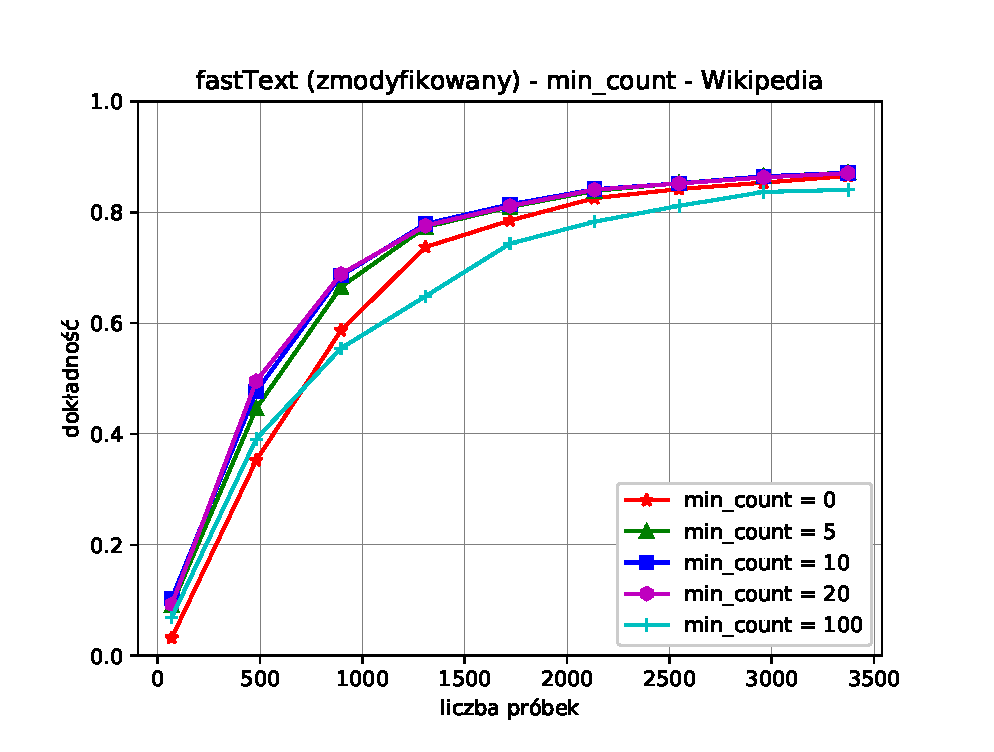
\includegraphics[width=0.45\linewidth]{img/fasttext-min_count-wikipedia}}}
    \qquad
    \subfloat[Wikipedia (rzeczowniki)]{{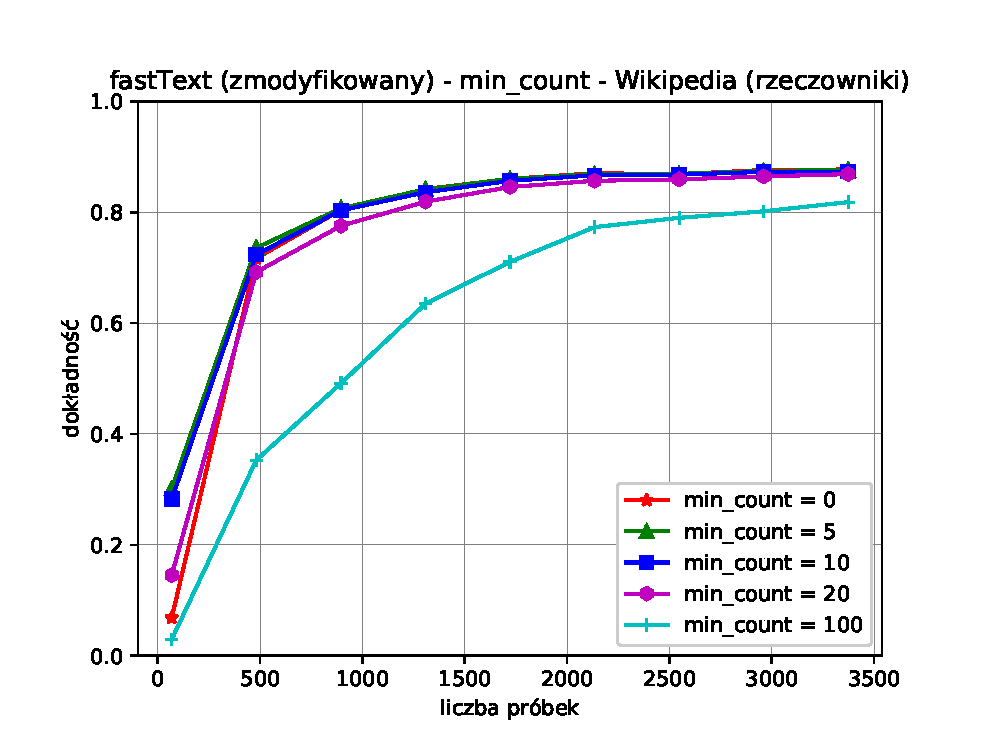
\includegraphics[width=0.45\linewidth]{img/fasttext-min_count-wikipedia-nouns}}}
    
	\caption{Porównanie wyników zmiany parametru \textit{min\_count}}
    \label{fig:fasttext-mincount}
\end{figure}

Wyniki dla 5 testowanych wartości zbiegają do tego samego poziomu. Najwięcej próbek potrzebował algorytm w przypadku parametru \textit{min\_count=100}. Początkowe wyniki na przedstawionych rysunkach \ref{fig:fasttext-mincount} wyraźnie pokazują, że najlepszą wartością w tym przypadku jest wartość 20. Dla korpusów z rzeczownikami można zaobserwować zmniejszenie się różnic w wynikach jakościowych pomiędzy wartościami: 0, 5, 10 oraz 20.
\newpage
\subsubsection{Zmiana parametru \textit{loss}}
Do wyboru są trzy różne wartości, które definiują który klasyfikator zostanie użyty podczas pracy. Domyślnym klasyfikatorem dla \textit{fastText} jest \textit{softmax} \cite{walkowiak2018}.

\begin{figure}[ht!]
	\centering    
    \subfloat[Artykuły]{{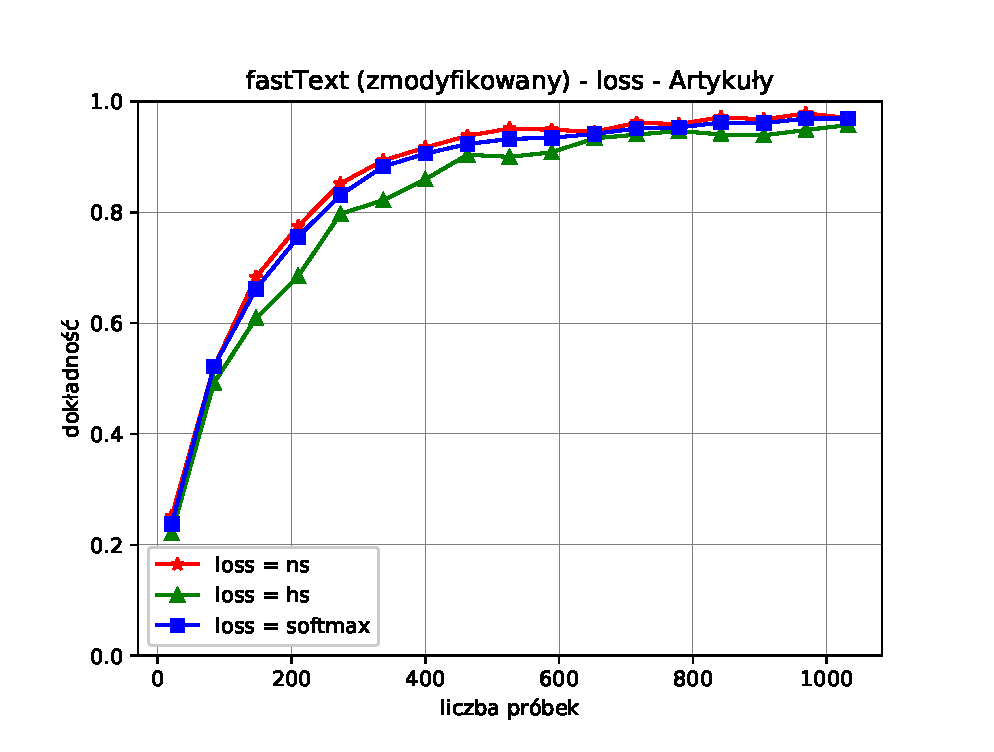
\includegraphics[width=0.45\linewidth]{img/fasttext-loss-articles}}}
    \qquad
    \subfloat[Artykuły (rzeczowniki)]{{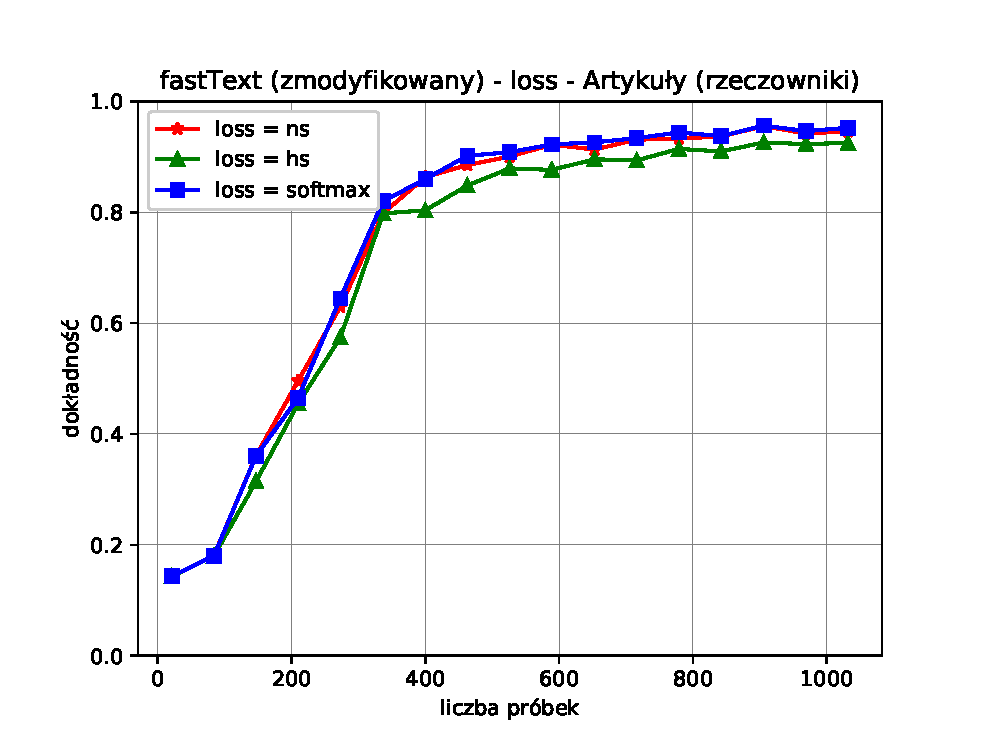
\includegraphics[width=0.45\linewidth]{img/fasttext-loss-articles-nouns}}}
    
    \subfloat[Wikipedia]{{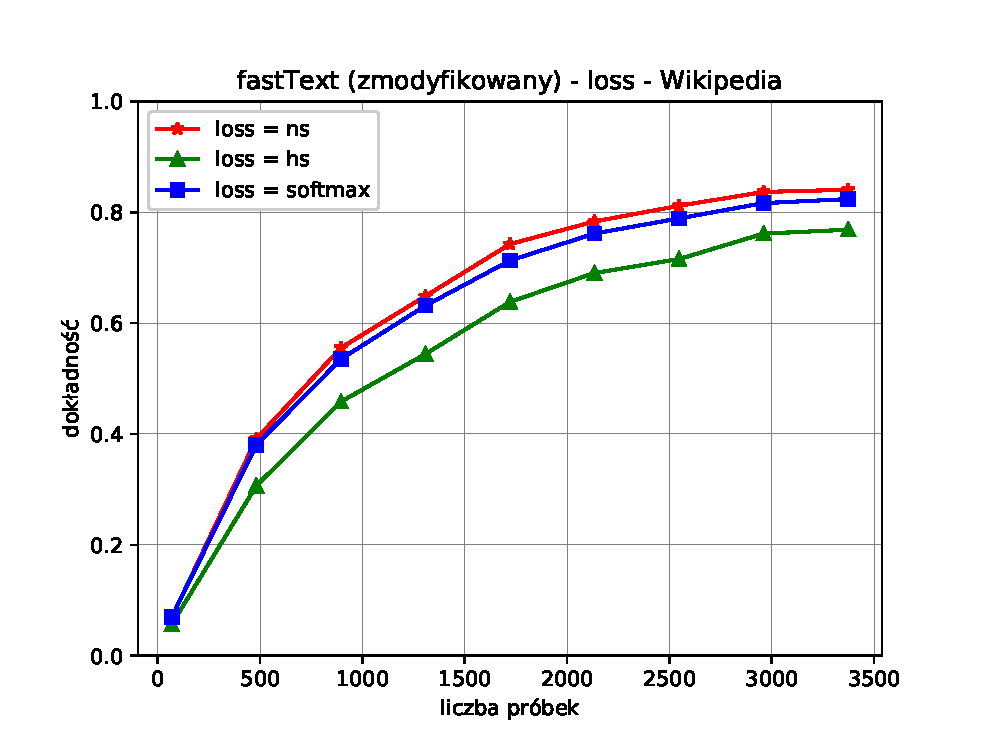
\includegraphics[width=0.45\linewidth]{img/fasttext-loss-wikipedia}}}
    \qquad
    \subfloat[Wikipedia (rzeczowniki)]{{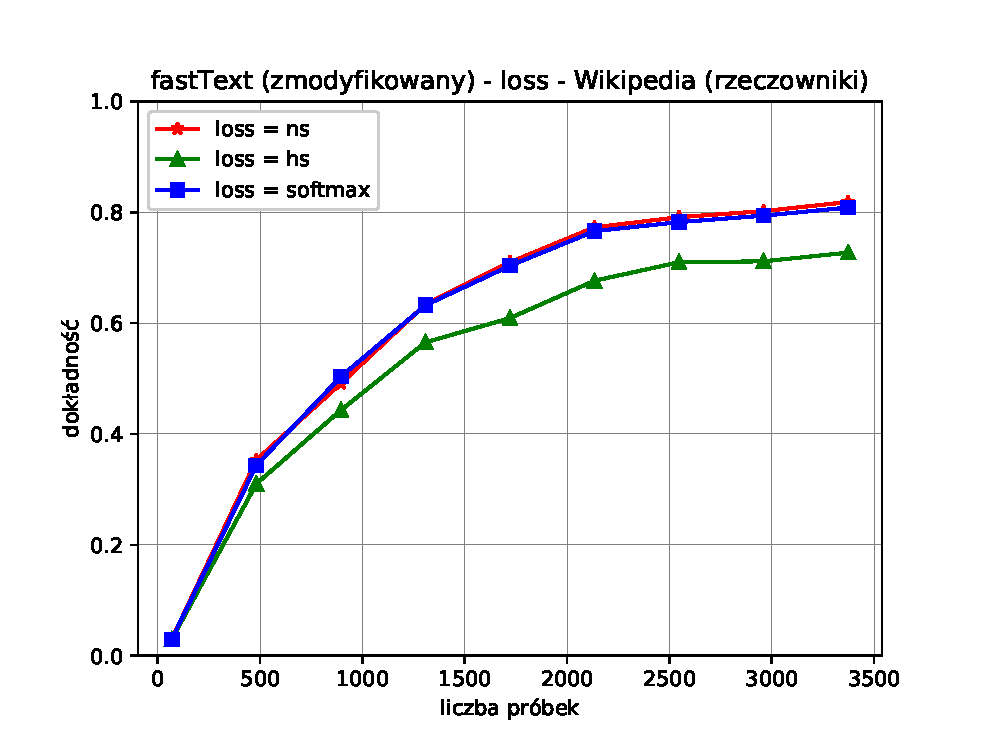
\includegraphics[width=0.45\linewidth]{img/fasttext-loss-wikipedia-nouns}}}
    
	\caption{Porównanie wyników zmiany parametru \textit{loss}}
    \label{fig:fasttext-loss}
\end{figure}

Zmiana parametru \textit{loss} nie powodowała tak dużych zmian w wynikach jak poprzednie parametry. Jednoznacznie jednak można stwierdzić, że przy mniejszej ilości próbek algorytm \textit{softmax} zwraca lepsze wyniki niż pozostałe dwie metody. Ostatecznie najlepsze wyniki w przypadku użytego korpusu osiągnięto przy pomocy algorytmu \textit{ns (negative samples)} i to on zostanie użyty w końcowych testach porównawczych. Wyniki na wykresach zostały przedstawione na rysunku \ref{fig:fasttext-loss}.

\newpage
\subsubsection{Zmiana parametru \textit{epoch}}

Parametr \textit{epoch} oznacza liczbę iteracji, które musi wykonać algorytm, aby nauczyć się korpusu \cite{fasttext-github}. Liczba iteracji jest tożsama z liczbą możliwości zobaczenia przez \textit{fastText} konkretnego dokumentu. 

\begin{figure}[ht!]
	\centering    
    \subfloat[Artykuły]{{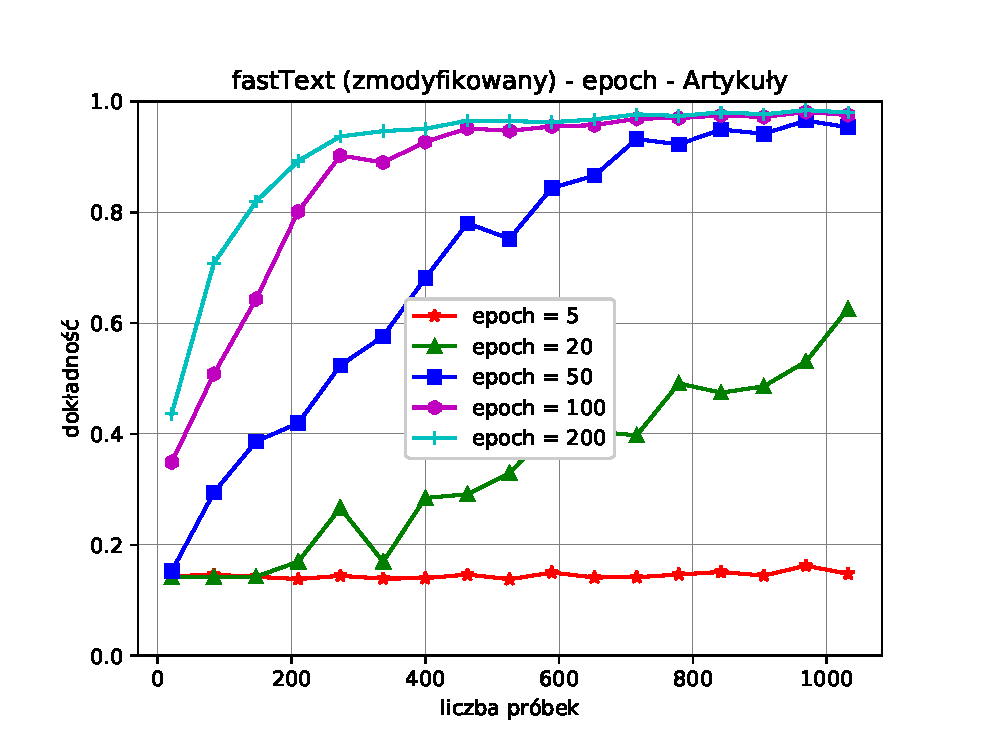
\includegraphics[width=0.45\linewidth]{img/fasttext-epoch-articles}}}
    \qquad
    \subfloat[Artykuły (rzeczowniki)]{{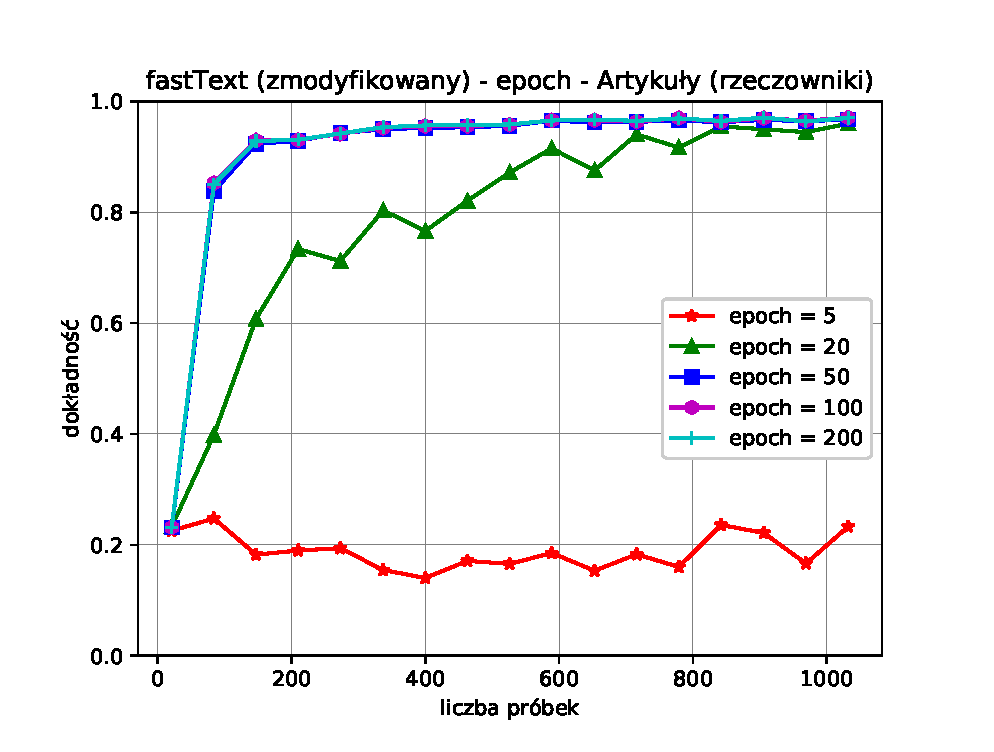
\includegraphics[width=0.45\linewidth]{img/fasttext-epoch-articles-nouns}}}
    
    \subfloat[Wikipedia]{{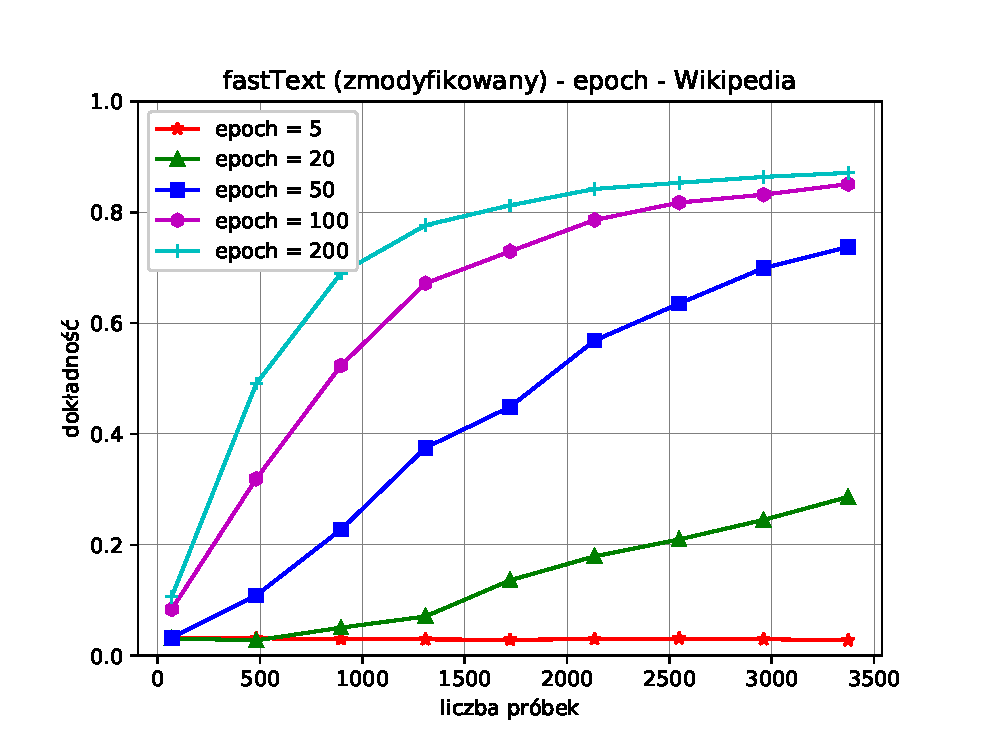
\includegraphics[width=0.45\linewidth]{img/fasttext-epoch-wikipedia}}}
    \qquad
    \subfloat[Wikipedia (rzeczowniki)]{{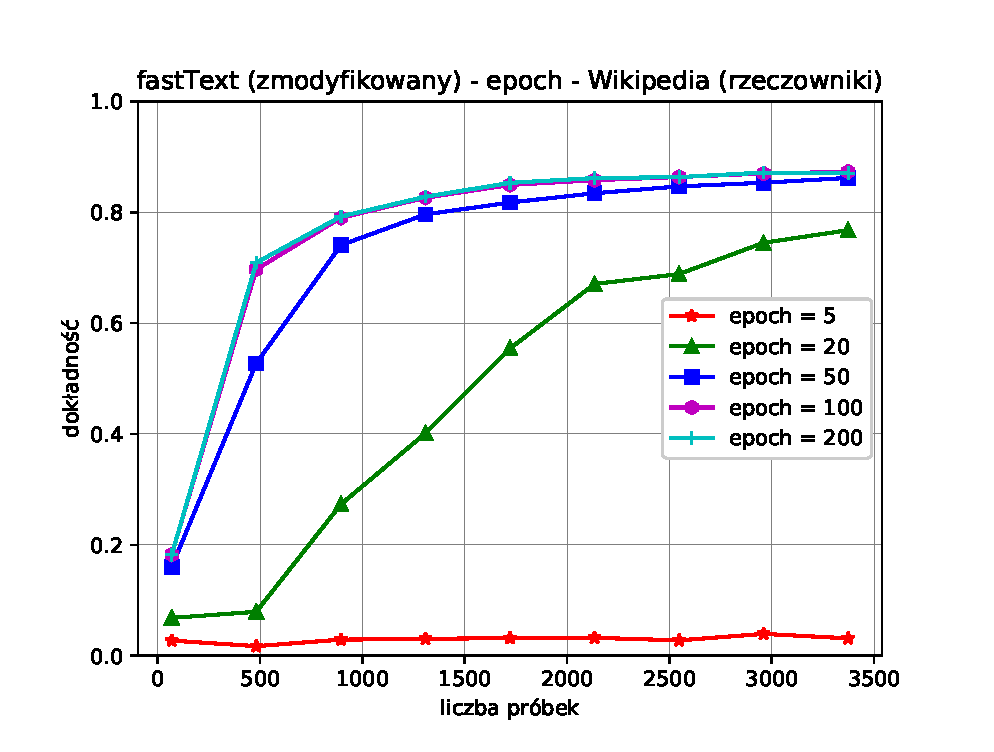
\includegraphics[width=0.45\linewidth]{img/fasttext-epoch-wikipedia-nouns}}}
    
	\caption{Porównanie wyników zmiany parametru \textit{epoch}}
    \label{fig:fasttext-epoch}
\end{figure}

Domyślną wartością parametru \textit{epoch} w \textit{fastText} jest wartość 5 i w przypadku wykorzystanych korpusów zwracane wyniki są bardzo niskie, niezależnie od ilości próbek. Najlepsze wyniki osiągnięto przy użyciu wyższych wartości, kosztem czego jest dłuższy czas nauki algorytmu, co jest oczekiwanym efektem. Wartości 50, 100 oraz 200 uzyskują zbliżone do siebie wyniki w przypadku korpusu z rzeczownikami, z widoczną korzyścią dla wartości 200 w pełnym korpusie. Wartości pośrednie - 50 oraz 20, wraz ze zwiększającą ilością danych testowych dąży do wyników osiąganych przez najlepsze wartości parametrów.

\subsubsection{Zmodyfikowane parametry}
Ostatecznie dobrano optymalne wartości dla każdego parametru i  przedstawiono je w tabeli \ref{tab:optimal-param}. Kolejne testy wykonano przy ich użyciu, a metodę określano jako \textit{fastText (zmodyfikowany)}.

\begin{table}[hb!]
\centering
\caption{Optymalne parametry biblioteki \textit{fastText} dla testowanych danych}
\label{tab:optimal-param}
\begin{tabular}{|c|c|c|c|}
\hline
ngram & min\_count & loss                  & epoch \\ \hline
1     & 20         & ns (negative samples) & 200   \\ \hline
\end{tabular}
\end{table}

\clearpage
\section{Porównanie wyników}

Podczas wyznaczania raportów jakości, dane treningowe stanowiły stosunek 70 do 30 dla obu testowanych korpusów. Składały się z 1820 dokumentów uczących oraz 780 dokumentów testujących, co stanowiło stosunek 70 do 30.
%%%%%%%%%%%%%%%%%%%%%%%%%%%%%%%%%%%%%%%%%%%%%%%%%%%%%%%%%%%%%%%%%%%%%%%%%%%%%%%%%%%%%%%%%%%%%%%%%%%%

\subsection{Analiza zbadanych miar}
Dla każdego klasyfikatora wygenerowana została tabela z wynikami miar dla każdej klasy w zbiorze dokumentów: \textit{precyzji (ang. precision)}, \textit{czułości (ang. recall)}, \textit{miary f1 (ang. f1-score)}. W ostatnim wierszu znajdują się wartości uśrednione oznaczone jako \textit{średnia}.


%%%%%%%%%%%%%%%%%%%%%%%%%%%%%%%%% NB
\subsubsection{Naive Bayes}
\begin{figure}[ht!]
	\centering
	\subfloat[Artykuły]{{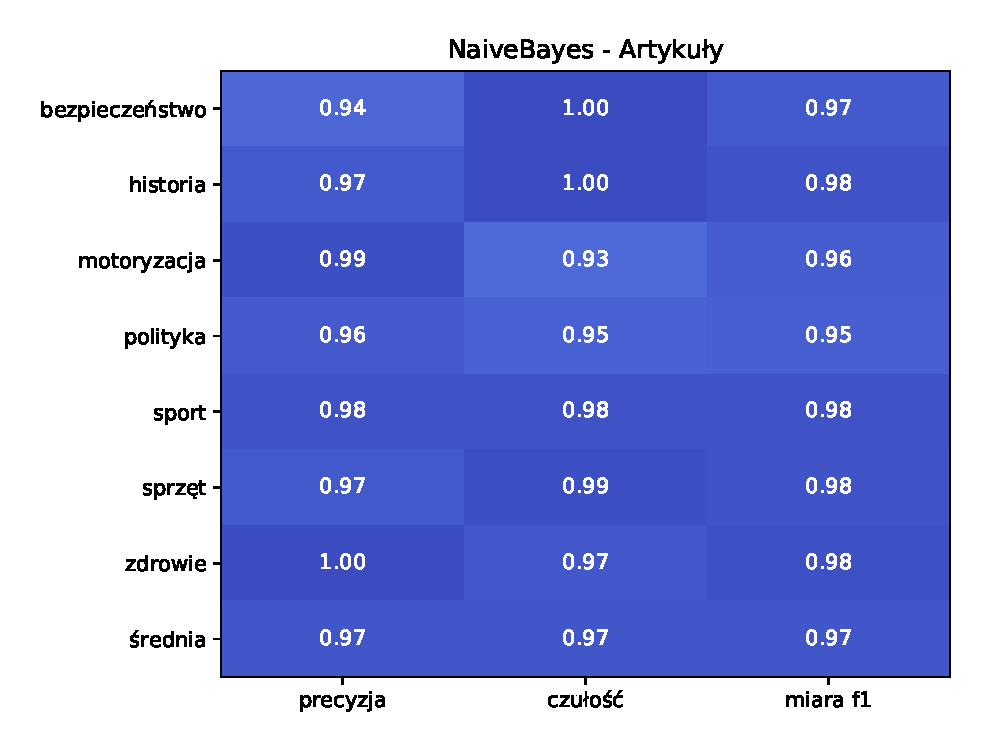
\includegraphics[width=0.45\linewidth]{img/report-naivebayes-articles}}}
    \qquad
    \subfloat[Artykuły (rzeczowniki)]{{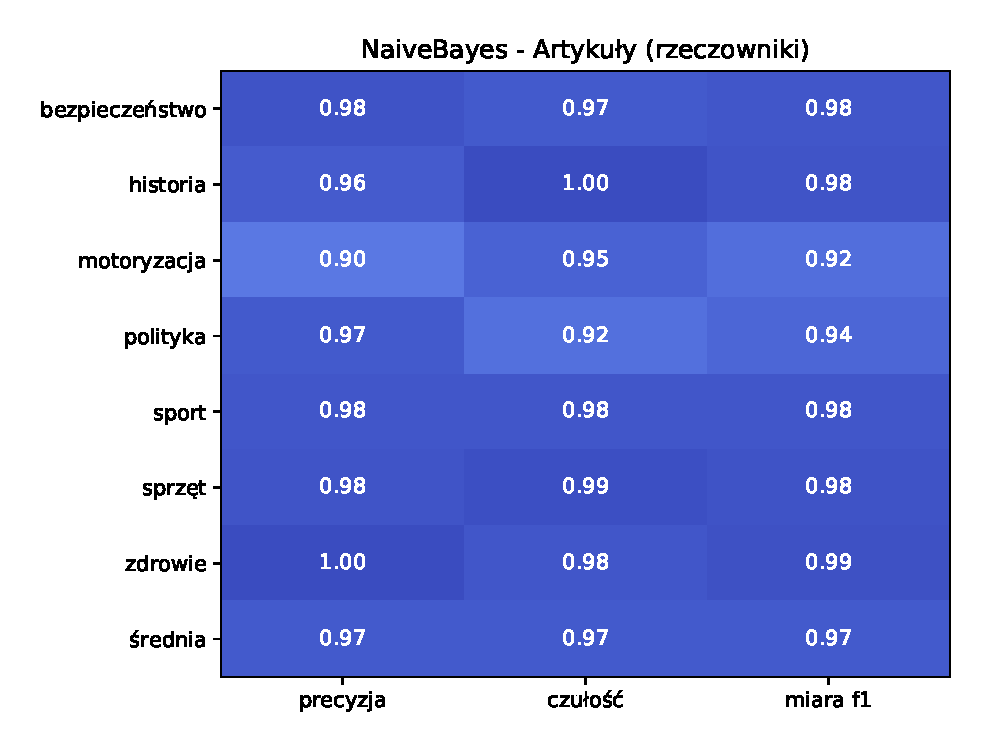
\includegraphics[width=0.45\linewidth]{img/report-naivebayes-articles-nouns}}}
	\caption{Miary jakościowe - NaiveBayes - Artykuły}
    \label{fig:report-naivebayes-articles}
\end{figure}
Rysunek \ref{fig:report-naivebayes-articles} przedstawia porównanie zbadanych miar dla pełnego korpusu oraz korpusu z samymi rzeczownikami. Według analizy skuteczność klasyfikatora \textit{NaiveBayes} w obu przypadkach jest zbliżona do siebie. Pojawiają się minimalne różnice na korzyść pełnych korpusów, co można zaobserwować w przypadku klasy \textit{zdrowie} oraz \textit{sprzęt}. Średnie wartości były takie same.

\begin{figure}[ht!]
	\centering
	\subfloat[Wikipedia]{{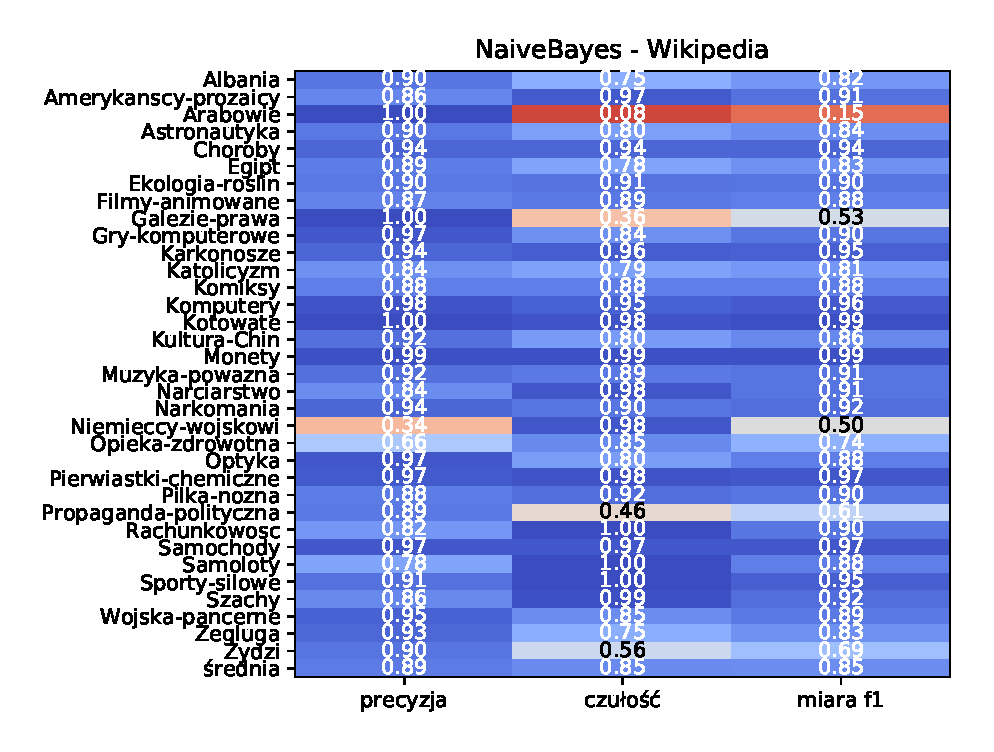
\includegraphics[width=0.45\linewidth]{img/report-naivebayes-wikipedia}}}
    \qquad
    \subfloat[Wikipedia (rzeczowniki)]{{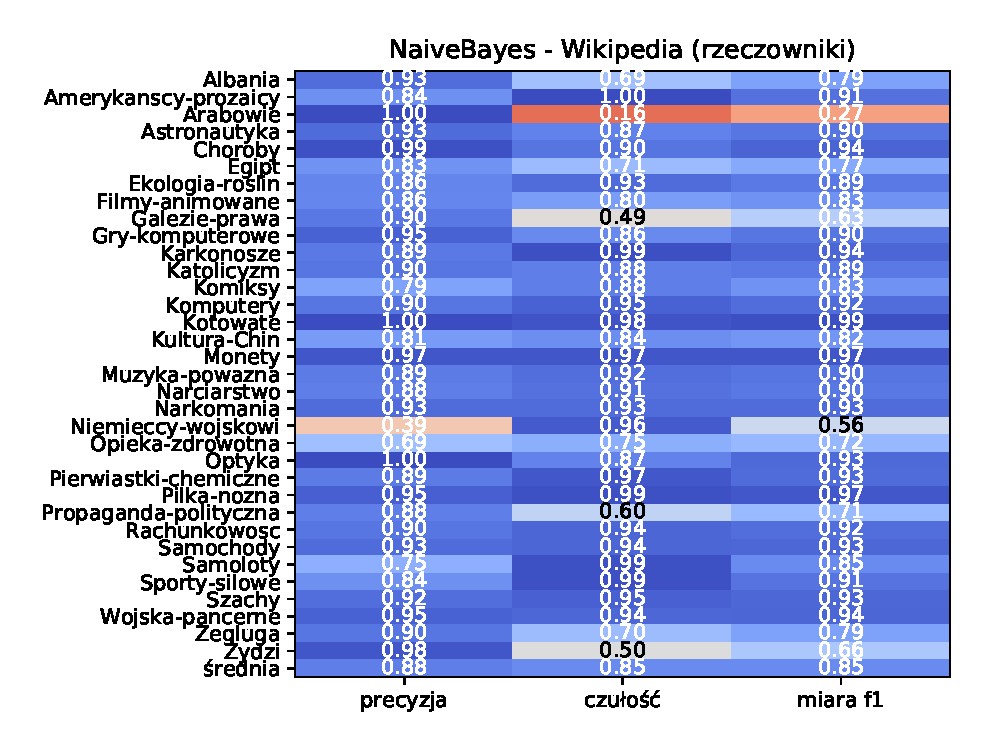
\includegraphics[width=0.45\linewidth]{img/report-naivebayes-wikipedia-nouns}}}
	\caption{Miary jakościowe - NaiveBayes - Wikipedia}
    \label{fig:report-naivebayes-wikipedia}
\end{figure}

Rysunek \ref{fig:report-naivebayes-wikipedia} przedstawia analogiczne porównanie zbiorów dla 34 klasowego korpusu Wikipedii. Średnie wyniki wskazują na to, że różnice pogłębiły się lecz wciąż były one bardzo małe. Wyniki miary f1 zostały bez zmian. Warto również zauważyć, że dla niektórych klas uzyskano lepsze wyniki; dobrym przykładem jest klasa \textit{propaganda-polityczna}, której wynik miary f1 poprawił się o 10 punktów procentowych w stosunku do pełnego korpusu. Mimo braku zmiany średniej wartości miary f1 widać poprawę w większości klas, które były słabo rozpoznawane. Wyjątkiem od reguły jest klasa \textit{kultura-chin}, której wynik czułości spadł o 4 punkty procentowe.

%%%%%%%%%%%%%%%%%%%%%%%%%%%%%%%%% SVM
\subsubsection{SVM}
\textit{SVM} uzyskał bardzo dobre wyniki we wszystkich przypadkach. Średnie wartości były najwyższe dla każdego typu testowanych danych dla badanych klasyfikatorów. 
\begin{figure}[ht!]
	\centering
	\subfloat[Artykuły]{{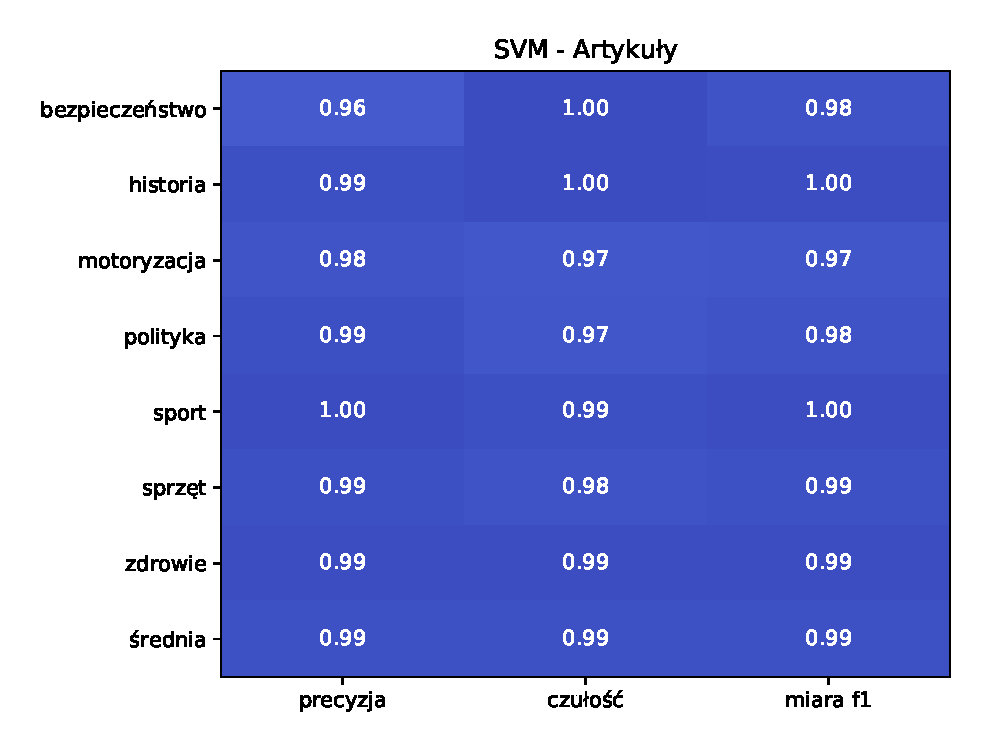
\includegraphics[width=0.45\linewidth]{img/report-svm-articles}}}
    \qquad
    \subfloat[Artykuły (rzeczowniki)]{{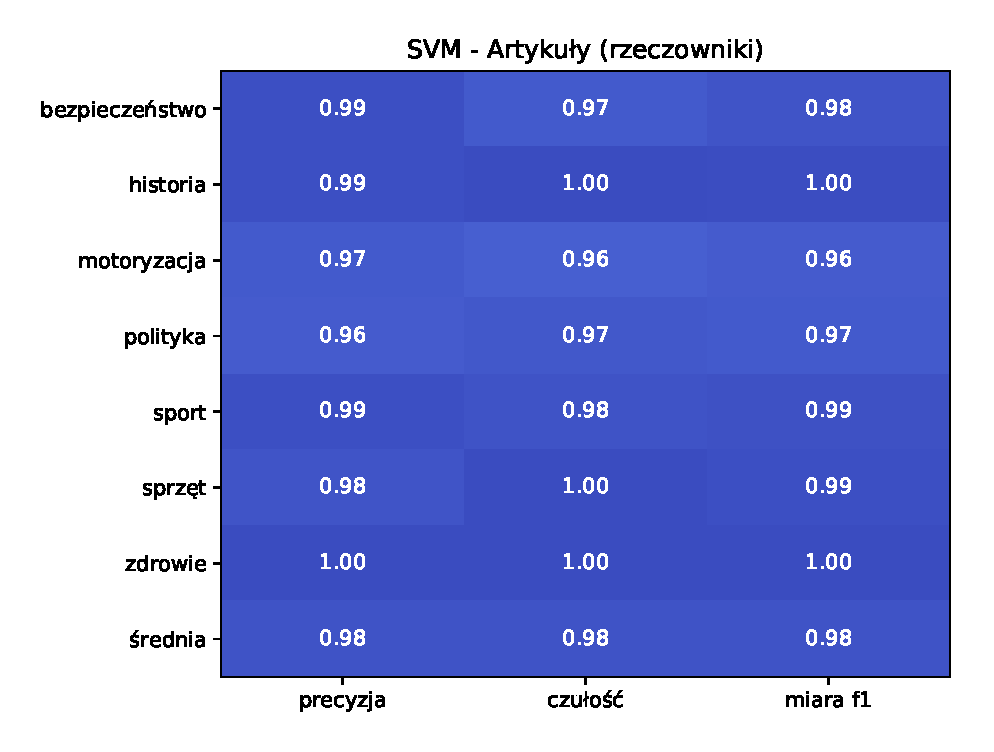
\includegraphics[width=0.45\linewidth]{img/report-svm-articles-nouns}}}
	\caption{Miary jakościowe - SVM - Artykuły}
    \label{fig:report-svm-articles}
\end{figure}

Wykresy na rysunku \ref{fig:report-svm-articles} jednoznacznie wskazują na bardzo dobre dopasowania każdej z klas. Najniższa zanotowana wartość miary była nie niższa niż 0.96; klasyfikator \textit{SVM} niemal bezbłędnie rozpoznawał wszystkie klasy. Dla tych dwóch zbiorów ocena, czy użycie samych rzeczowników pozytywnie wpływa na jakość klasyfikacji, byłaby nadinterpretacją lecz z całą pewnością można stwierdzić, że nie ma negatywnego wpływu na przypisywanie kategorii zadanym tekstom.  

\begin{figure}[ht!]
	\centering
	\subfloat[Wikipedia]{{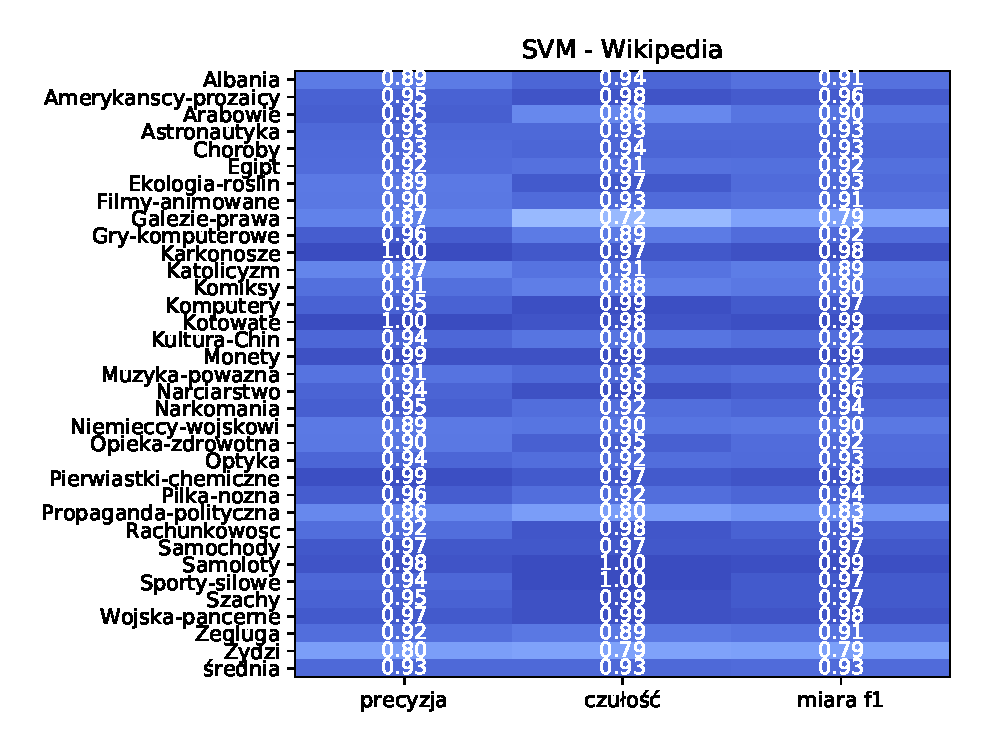
\includegraphics[width=0.45\linewidth]{img/report-svm-wikipedia}}}
    \qquad
    \subfloat[Wikipedia (rzeczowniki)]{{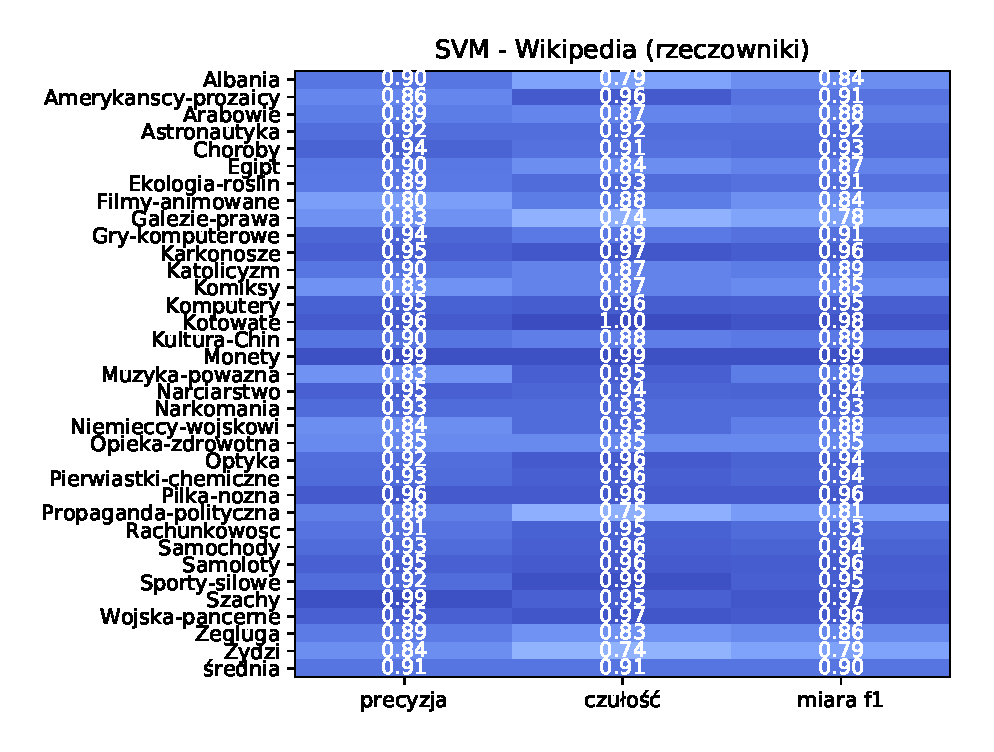
\includegraphics[width=0.45\linewidth]{img/report-svm-wikipedia-nouns}}}
	\caption{Miary jakościowe - SVM - Wikipedia}
    \label{fig:report-svm-wikipedia}
\end{figure}

Bardziej precyzyjne wnioski można otrzymać dopiero po analizie wyników na rysunku \ref{fig:report-svm-wikipedia}. Większa liczba klas wystarczająco utrudniła dopasowywanie kategorii, można zaobserwować, że średnie wyniki wszystkich rozpatrywanych miar pogorszyły się o 1/2 punkty procentowe. Słabo rozpoznawane kategorie z przedziału od 0.7 do 0.8 nie były lepiej dopasowywane w zbiorze dokumentów z samymi rzeczownikami.   

%%%%%%%%%%%%%%%%%%%%%%%%%%%%%%%%% DT 

\subsubsection{Drzewo decyzyjne}
\textit{Drzewo decyzyjne} osiągało najgorsze wyniki, ze wszystkich testowanych klasyfikatorów dla badanych zbiorów danych.
\begin{figure}[ht!]
	\centering
	\subfloat[Artykuły]{{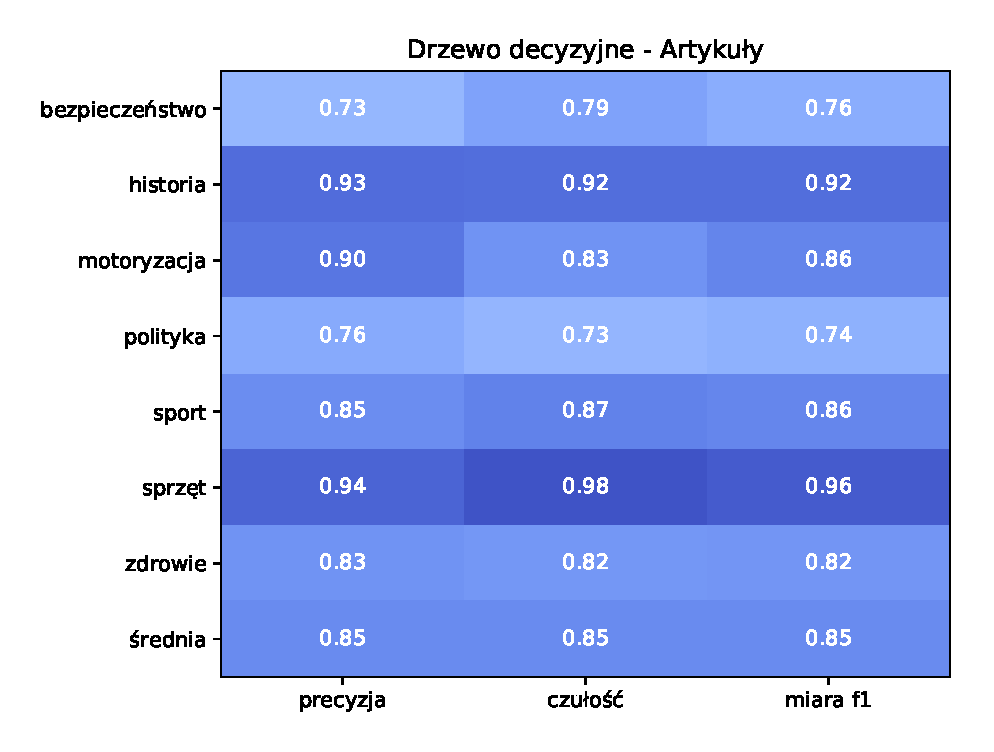
\includegraphics[width=0.45\linewidth]{img/report-decisiontree-articles}}}
    \qquad
    \subfloat[Artykuły (rzeczowniki)]{{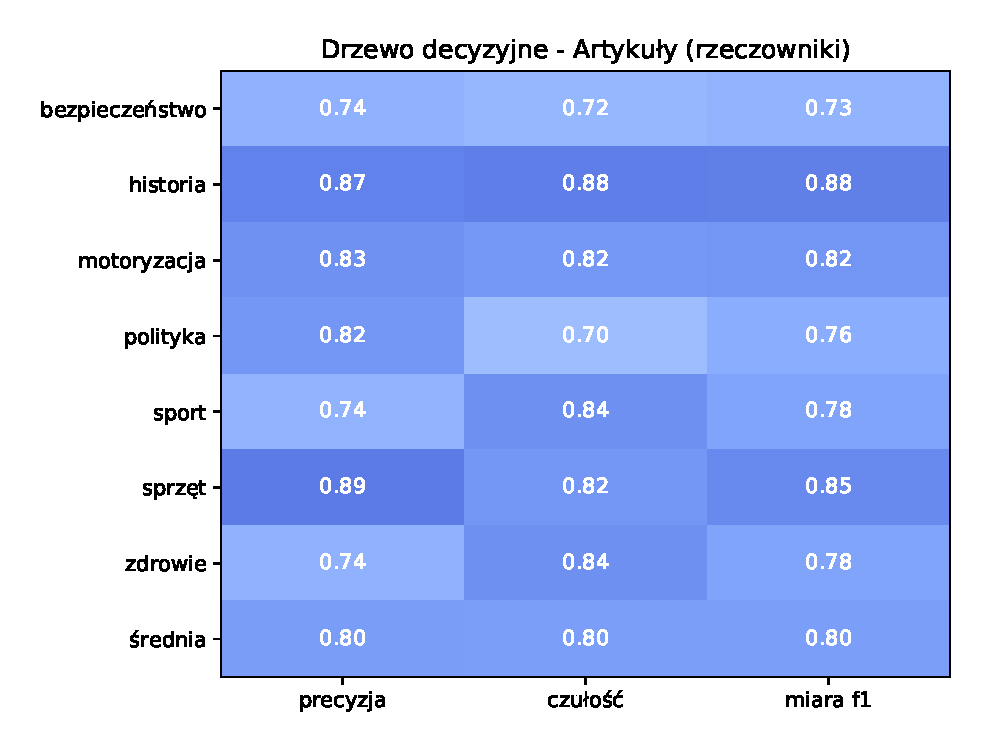
\includegraphics[width=0.45\linewidth]{img/report-decisiontree-articles-nouns}}}
	\caption{Miary jakościowe - Drzewo decyzyjne - Artykuły}
    \label{fig:report-dt-articles}
\end{figure}

Wszystkie kategorie uzyskały gorsze wyniki dla miary f1 po odrzuceniu innych części mowy niż rzeczowniki, o czym również świadczą niższe wartości średnie. Wysokie wskaźniki dla klasy \textit{sprzęt} są wynikiem bardzo charakterystycznych zbiorów słów występujących w tej kategorii, bowiem zawiera ona bardzo dużo nazw własnych, co zostało zobrazowane na rysunku \ref{fig:freq-ign-words}.

\begin{figure}[ht!]
	\centering
	\subfloat[Wikipedia]{{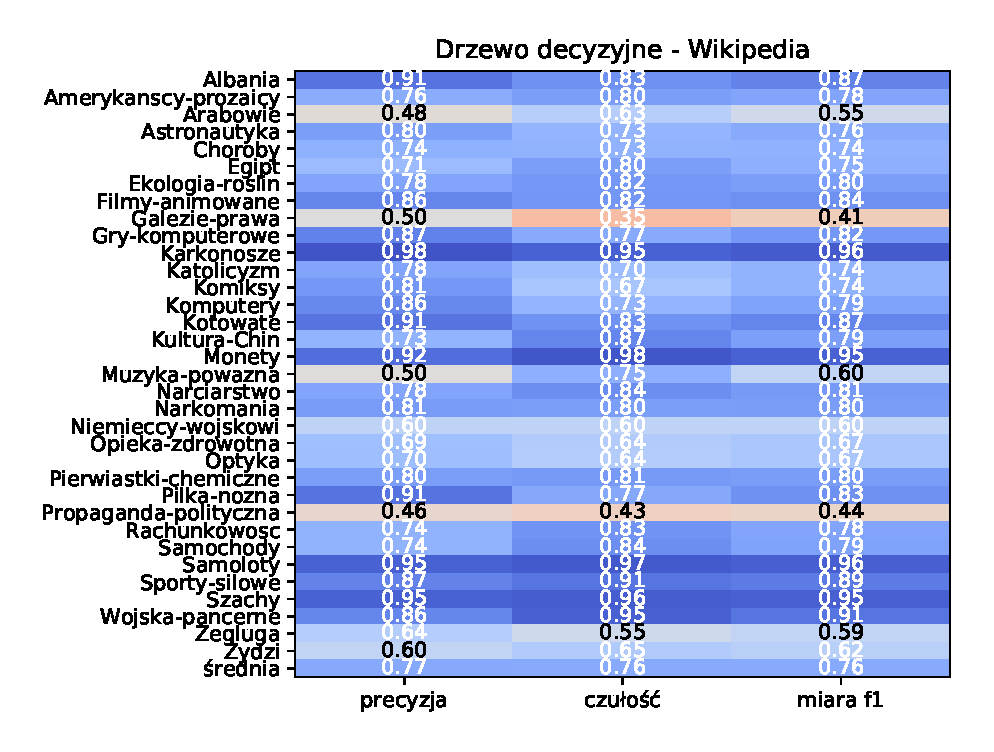
\includegraphics[width=0.45\linewidth]{img/report-decisiontree-wikipedia}}}
    \qquad
    \subfloat[Wikipedia (rzeczowniki)]{{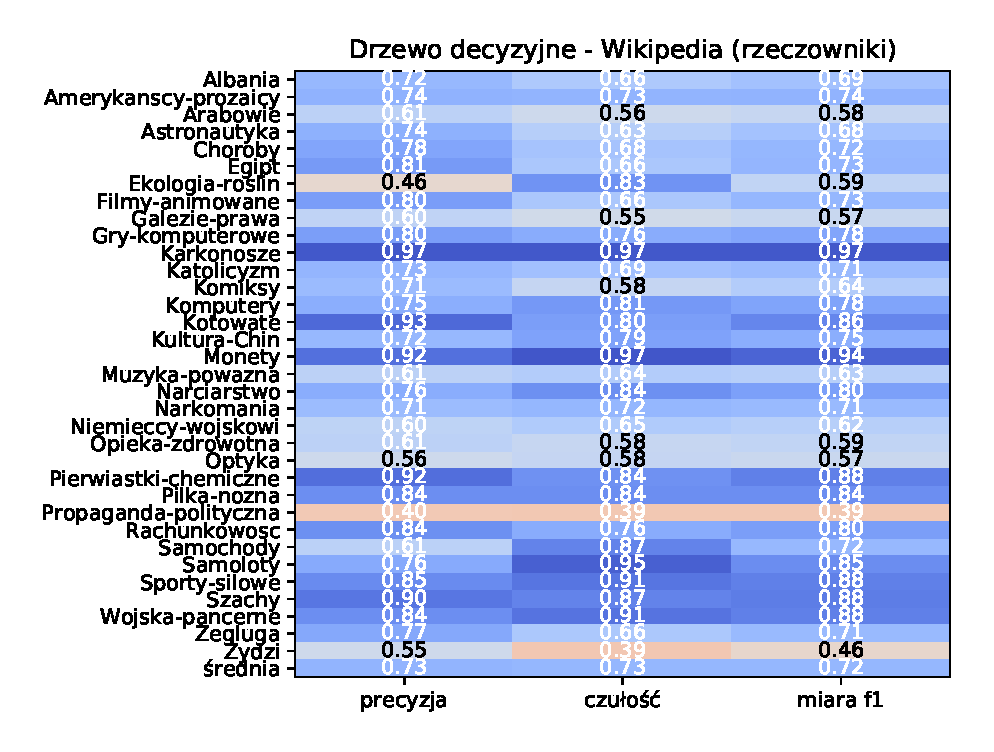
\includegraphics[width=0.45\linewidth]{img/report-decisiontree-wikipedia-nouns}}}
	\caption{Miary jakościowe - Drzewo decyzyjne - Wikipedia}
    \label{fig:report-dt-wikipedia}
\end{figure}

Ważnym wnioskiem po analizie rysunku \ref{fig:report-dt-wikipedia} jest fakt iż, klasyfikacja dla korpusu z rzeczownikami w większości pogłębiła różnice między korpusami. Słabe wyniki, poniżej wartości 0.7 miary f1, obniżyły się, a wysokie wyniki, powyżej 0.8, polepszyły. Przykładami takiego zachowania są klasy \textit{karkonosze} (polepszenie), \textit{żydzi} (pogorszenie), \textit{propaganda-polityczna} (pogorszenie), \textit{gałęzie-prawa} (pogorszenie)



%%%%%%%%%%%%%%%%%%%%%%%%%%%%%%%%% fastText
\clearpage
\subsubsection{fastText}
\textit{fastText} osiągał wyniki zbliżone do tych, które zwracały klasyfikatory \textit{NaiveBayes} oraz \textit{SVM}, co plasuje go na drugim miejscu pod względem jakości dopasowywanych klas na podstawie otrzymanych średnich wyników dla testowanych miar na badanych korpusach.  
\begin{figure}[ht!]
	\centering
	\subfloat[Artykuły]{{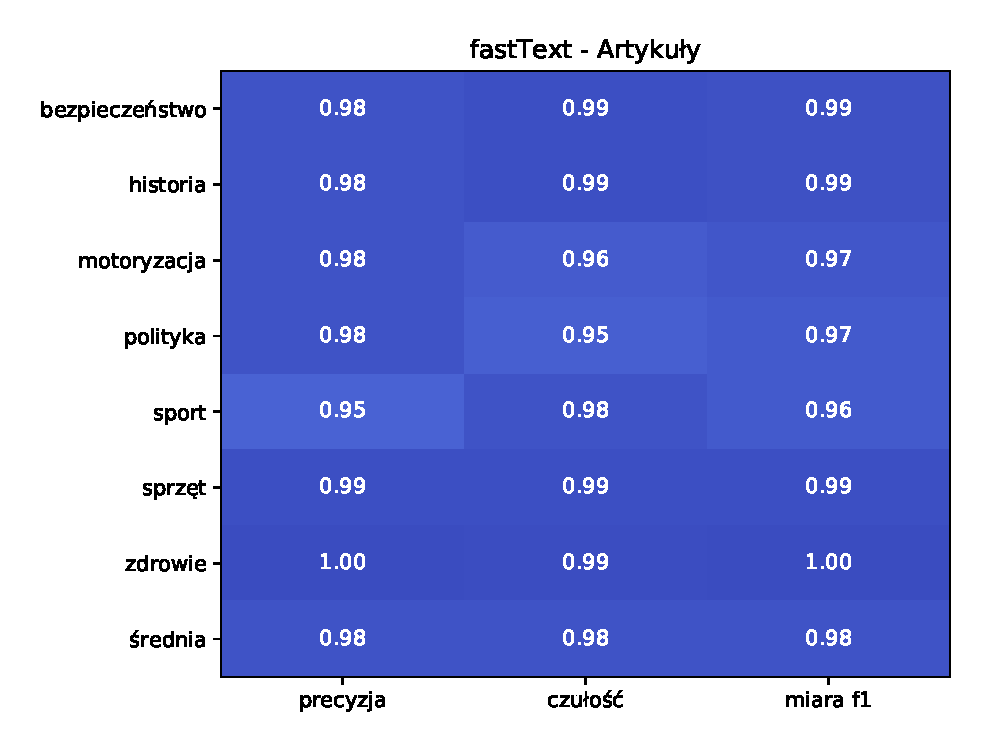
\includegraphics[width=0.45\linewidth]{img/report-fasttext-articles}}}
    \qquad
    \subfloat[Artykuły (rzeczowniki)]{{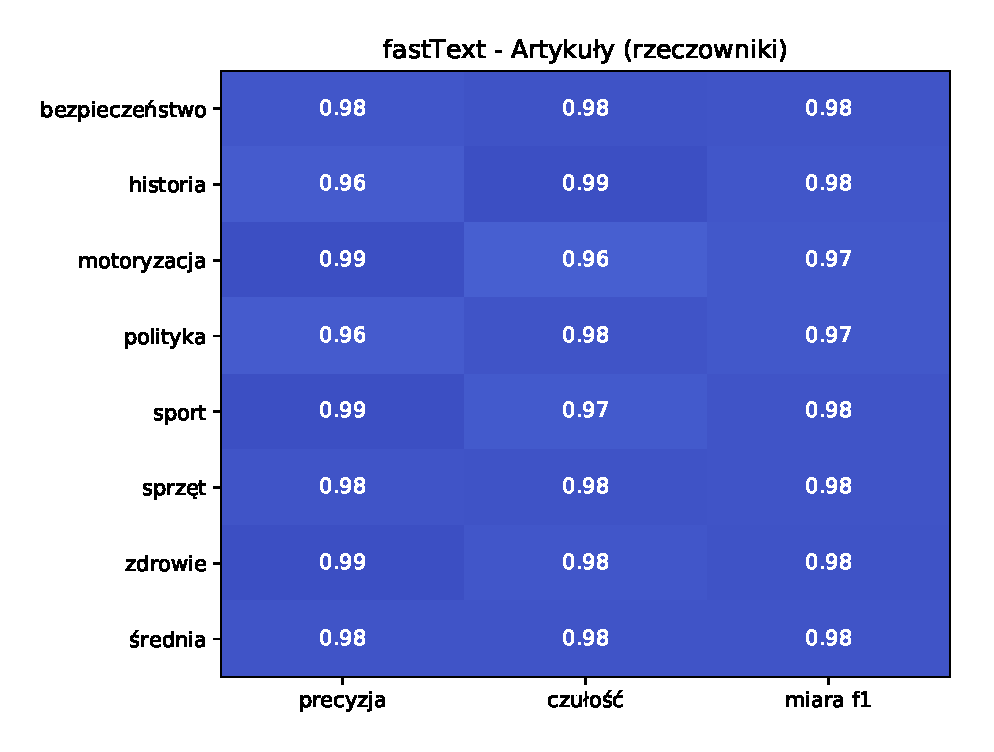
\includegraphics[width=0.45\linewidth]{img/report-fasttext-articles-nouns}}}
	\caption{Miary jakościowe - fastText - Artykuły}
    \label{fig:report-fasttext-articles}
\end{figure}

\textit{fastText} bardzo dobrze klasyfikował artykuły w obu przypadkach, co pokazuje rysunek \ref{fig:report-fasttext-articles}. Nie utracił on znacznie skuteczności w jakości działania, mimo ograniczania zbioru dokumentów do samych rzeczowników. 

\begin{figure}[ht!]
	\centering
	\subfloat[Wikipedia]{{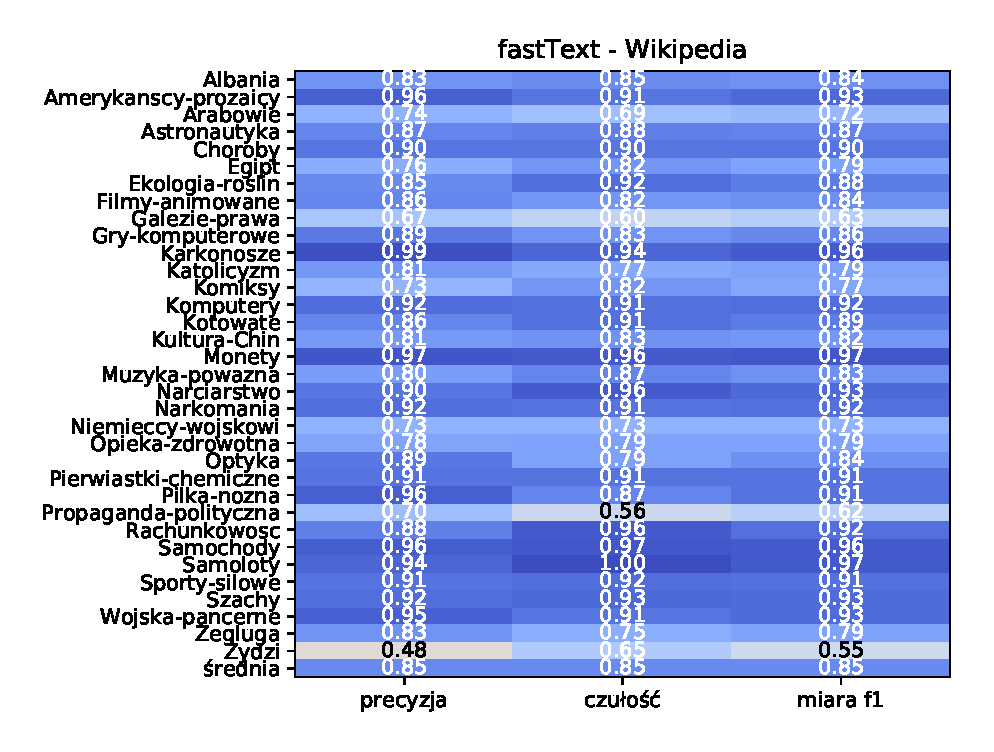
\includegraphics[width=0.45\linewidth]{img/report-fasttext-wikipedia}}}
    \qquad
    \subfloat[Wikipedia (rzeczowniki)]{{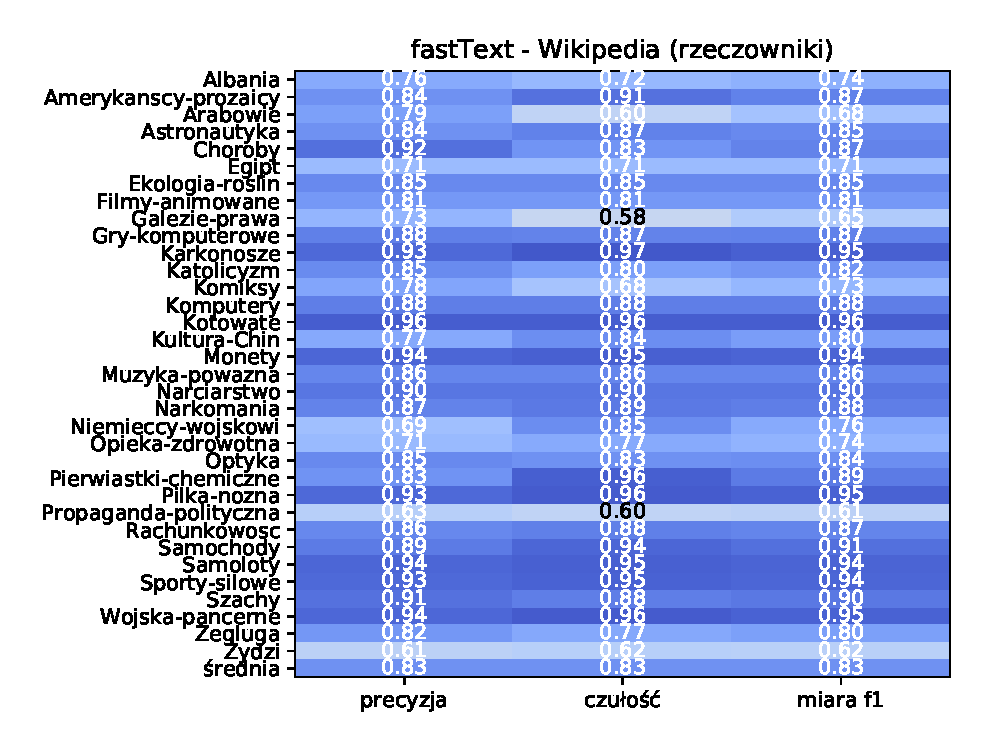
\includegraphics[width=0.45\linewidth]{img/report-fasttext-wikipedia-nouns}}}
	\caption{Miary jakościowe - fastText - Wikipedia}
    \label{fig:report-fasttext-wikipedia}
\end{figure}

Pełniejszy obraz dało przebadanie klasyfikatora na zbiorze danych z większą liczbą klas. Podobnie jak w pozostałych przypadkach, końcowe wartości średnie nieznacznie obniżyły się, co można uznać za regułę niezależnie od ilości danych i rodzaju użytego klasyfikatora badanego w pracy.

\subsubsection{Wnioski}
Na podstawie przebadanych klasyfikatorów i analizie badanych miar, podstawowym wnioskiem jaki należy wysnuć jest fakt, iż w każdym przypadku jakość klasyfikacji nieznacznie obniża się o około kilka punktów procentowych dla wszystkich miar lub pozostaje bez zmian. Jest to oczekiwany wynik \cite{walkowiak2018} obniżenia się jakości wyników. 
Bardzo niskie wartości miar dla drzewa decyzyjnego w stosunku do innych klasyfikatorów pozwoliły na stwierdzenie pewnej zależności między pełnym korpusem, a korpusem z rzeczownikami. W wielu przypadkach, gdzie dopasowanie klasy w pełnym korpusie jest niskie, widać pogorszenie się tego wyniku dla samych rzeczowników. Natomiast jeśli wartość miary f1 jest wysoka dla pełnego korpusu, wynik będzie wyższy dla samych rzeczowników. Reguła ta najbardziej widoczna jest w klasyfikatorach \textit{NaiveBayes} oraz \textit{drzewo decyzyjne}. 
Trudno jednak przyjąć taki wniosek za regułę, gdyż istnieją również odstępstwa; na przykład klasa \textit{propaganda-polityczna} w \textit{drzewie decyzyjnym}, w której po wykonaniu testów na zbiorze z samymi rzeczownikami wynik wzrósł w przeciwieństwie do bardzo niskiego wyniku miary f1 0.45 w pełnym zbiorze.

%%%%%%%%%%%%%%%%%%%%%%%%%%%%%%%%%%%%%%%%%%%%%%%%%%%%%%%%%%%%%%%%%%%%%%%%%%%%%%%%%%%%%%%%%%%%%%%%%%%%

\subsection{Analiza macierzy błędów}
Macierze błędów pozwalają na graficzne przedstawienie klas, w których najczęściej występowały błędy. Dla każdego klasyfikatora została wygenerowano macierz pomyłek. Podczas analizy pominięto analizę macierzy, które nie zawierały znacznych błędów. Macierz na osi x zawiera klasy, które powinny zostać dopasowane oznaczone (\textit{dopasowana klasa}), natomiast na osi y znajdują się klasy, które przyporządkował klasyfikator (\textit{rzeczywista klasa}). Macierz, która zawiera mało pomyłek, charakteryzuje się wartościami wysokimi i ciemnymi polami po przekątnej, oznacza to, że klasyfikator poprawnie dopasował kategorię do zadanego tekstu.

\subsubsection{Drzewo decyzyjne}

\begin{figure}[ht!]
	\centering
	\subfloat[Artykuły]{{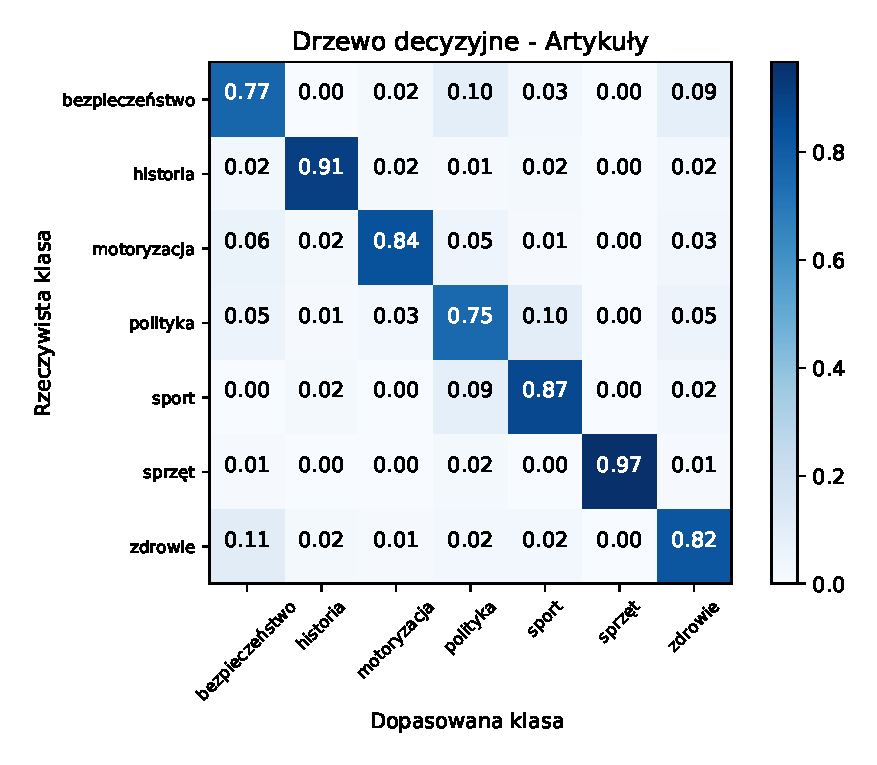
\includegraphics[width=0.45\linewidth]{img/c-matrix-decisiontree-articles}}}
    \qquad
    \subfloat[Artykuły (rzeczowniki)]{{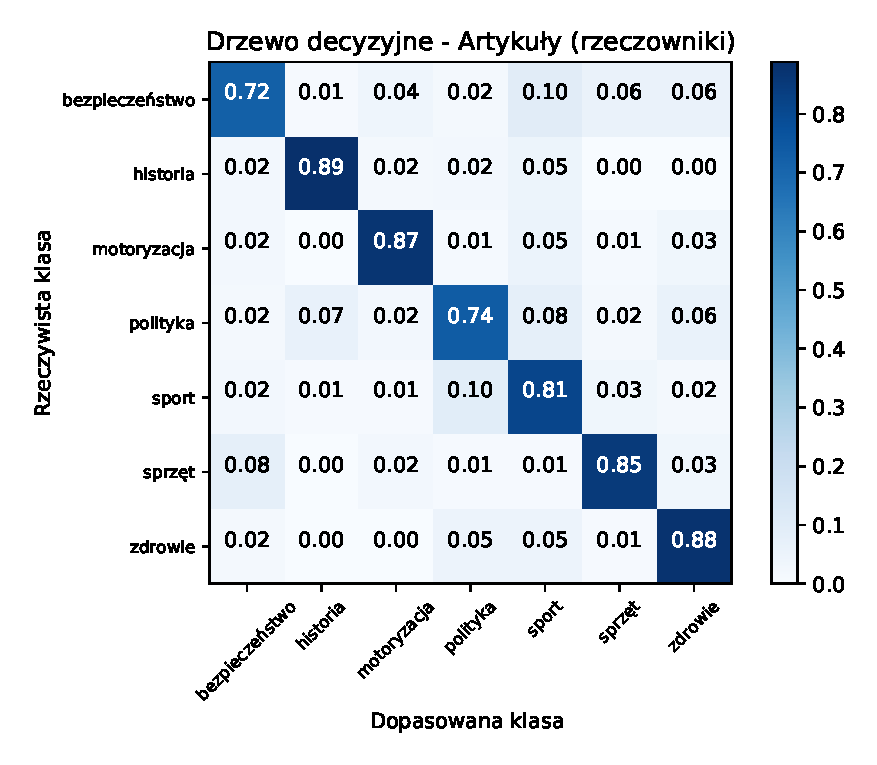
\includegraphics[width=0.45\linewidth]{img/c-matrix-decisiontree-articles-nouns}}}
	\caption{Tablica pomyłek - Drzewo decyzyjne - Artykuły}
    \label{fig:c-matrix-dt-articles}
\end{figure}
Drzewo decyzyjne osiągało najgorsze wyniki, więc analiza jego tablicy pomyłek jest bardzo istotna. Można zauważyć pewną anomalię dla korpusu z rzeczownikami: klasyfikator próbował dopasować kategorię \textit{polityka} do klas \textit{bezpieczeństwo}, \textit{zdrowie}, \textit{sport}, \textit{historia}. 
Jedną z częściej mylonych klas była kategoria \textit{polityka} i klasyfikator często  mylił ją z kategorią \textit{bezpieczeństwo} (10\% przypadków) oraz \textit{zdrowie} (9\% przypadków) w pełnym korpusie. Wysoką wartość dla klasy \textit{bezpieczeństwo} można tłumaczyć faktem, że obie kategorie poruszają tematy istotne dla bezpieczeństwa i społeczeństwa. 6-procentową wartość błędu dla klasy \textit{sprzęt} w przypadku korpusu z rzeczownikami można tłumaczyć tym, że artykuły z klasy \textit{bezpieczeństwo} pochodziły głównie ze stron o bezpieczeństwie IT, występowanie podobnego słownictwa w obu tych kategoriach może być źródłem pomyłek. Na uwagę również zasługuje fakt, iż w korpusie ze wszystkimi klasami gramatycznymi taka anomalia nie występuje, więc dodatkowe klasy gramatyczne skutecznie stłumiły niepasujące cechy.
% * <jakub.pomykala@gmail.com> 2018-06-10T22:30:02.454Z:
% 
% > Najczęściej myloną klasą była kategoria \textit{bezpieczeństwo} i klasyfikator często  mylił ją z kategorią \textit{bezpieczeństwo}
% coś tu nie gra chyba
% 
% ^.
\begin{figure}[ht!]
	\centering
	\subfloat[Wikipedia]{{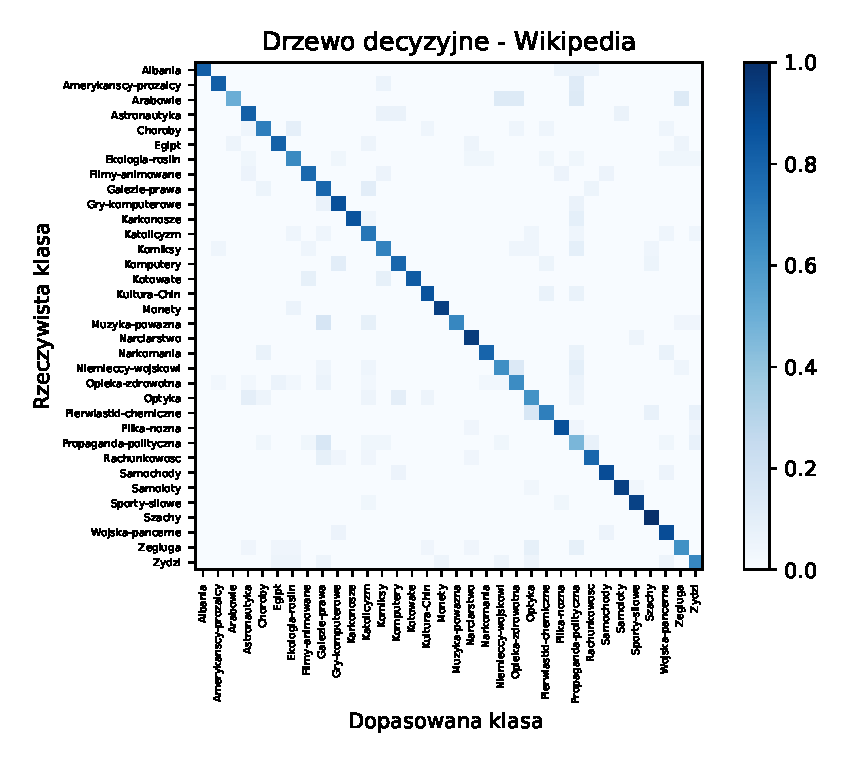
\includegraphics[width=0.45\linewidth]{img/c-matrix-decisiontree-wikipedia}}}
    \qquad
    \subfloat[Wikipedia (rzeczowniki)]{{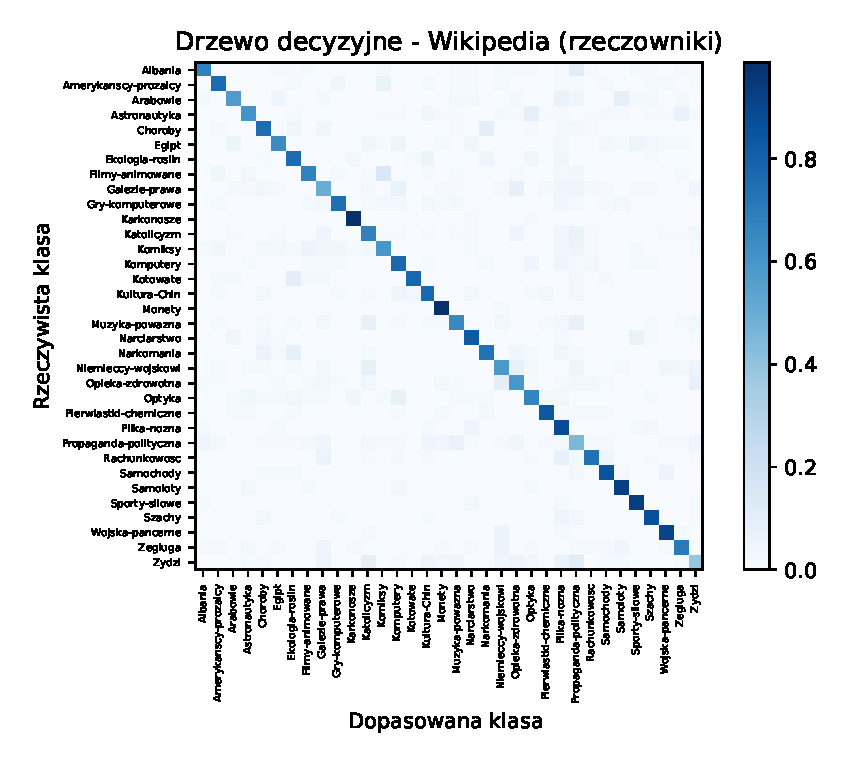
\includegraphics[width=0.45\linewidth]{img/c-matrix-decisiontree-wikipedia-nouns}}}
	\caption{Tablica pomyłek - Drzewo decyzyjne - Wikipedia}
    \label{fig:c-matrix-dt-wikipedia}
\end{figure}
W przypadku bardziej zróżnicowanego korpusu można dostrzec podobną sytuację dla klasy \textit{propaganda-polityczna}. Klasyfikator częściej niż inne próbował dopasować tę kategorię do wszystkich pozostałych kategorii.

\subsubsection{Naive Bayes}
\textit{NaiveBayes} mimo osiągnięcia najlepszych wyników,  nie wszystkie klasy były dopasowywane z wysokim prawdopodobieństwem.
\begin{figure}[ht!]
	\centering
	\subfloat[Wikipedia]{{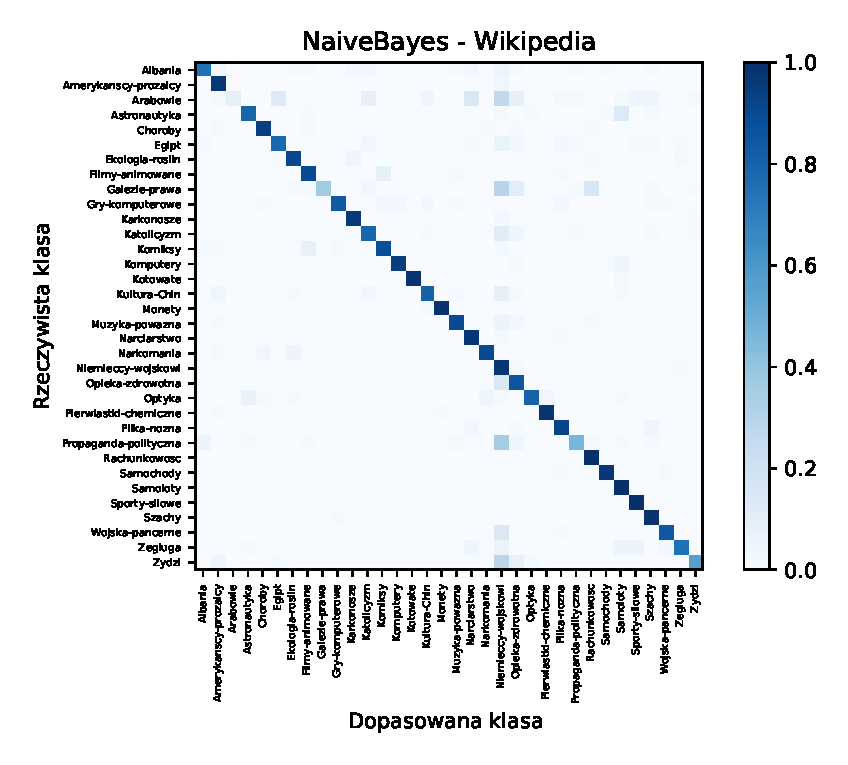
\includegraphics[width=0.45\linewidth]{img/c-matrix-naivebayes-wikipedia}}}
    \qquad
    \subfloat[Wikipedia (rzeczowniki)]{{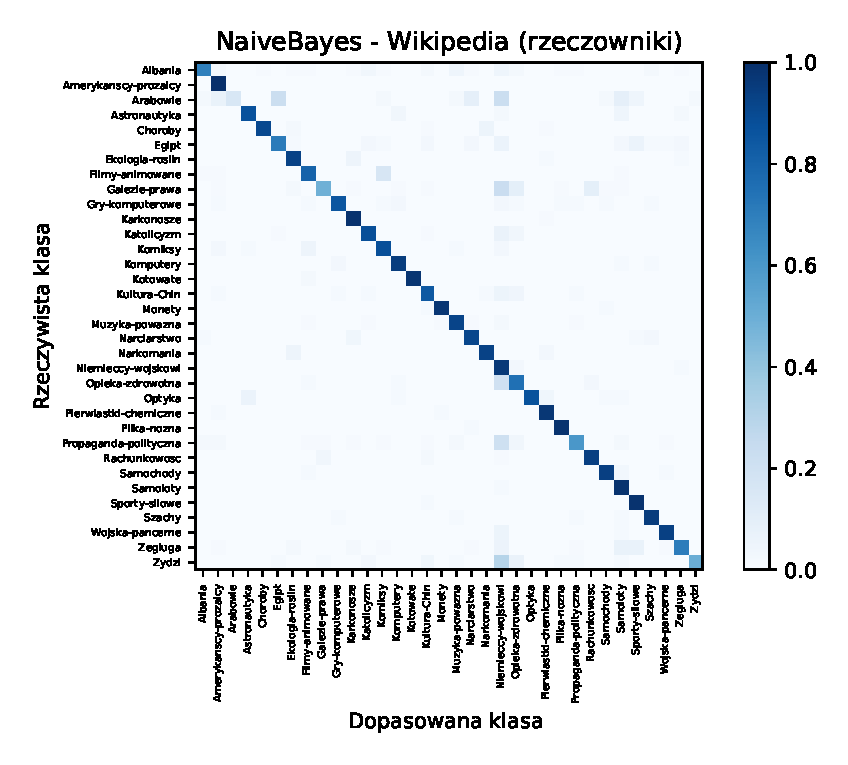
\includegraphics[width=0.45\linewidth]{img/c-matrix-naivebayes-wikipedia-nouns}}}
	\caption{Tablica pomyłek - Naive Bayes - Wikipedia}
    \label{fig:c-matrix-naivebayes-wikipedia}
\end{figure}

Dla korpusu z rzeczownikami liczba błędnych dopasowań zmniejszyła się lecz mimo to, pewna charakterystyka w obu przypadkach została zachowana. Klasa \textit{niemieccy-wojskowi} często była dopasowywana zamiast kategorii \textit{żydzi}, \textit{propaganda-polityczna}, \textit{gałęzie-prawa}, \textit{arabowie}. Sama klasa \textit{arabowie} jest bardzo słabo rozpoznawana i wykres na rysunku \ref{fig:c-matrix-naivebayes-wikipedia} pokazuje, że często była mylona z kategorią \textit{egipt}, \textit{narciarstwo}, \textit{niemieccy-wojskowi}, \textit{samoloty}. Klasyfikacja dla \textit{gałęzi-prawa} poprawiła się po odrzuceniu wyrazów innych niż rzeczowniki, głównie za sprawą lepszego rozpoznawania kategorii \textit{niemieccy-wojskowi}.

\begin{figure}[ht!]
	\centering
	\subfloat[Artykuły]{{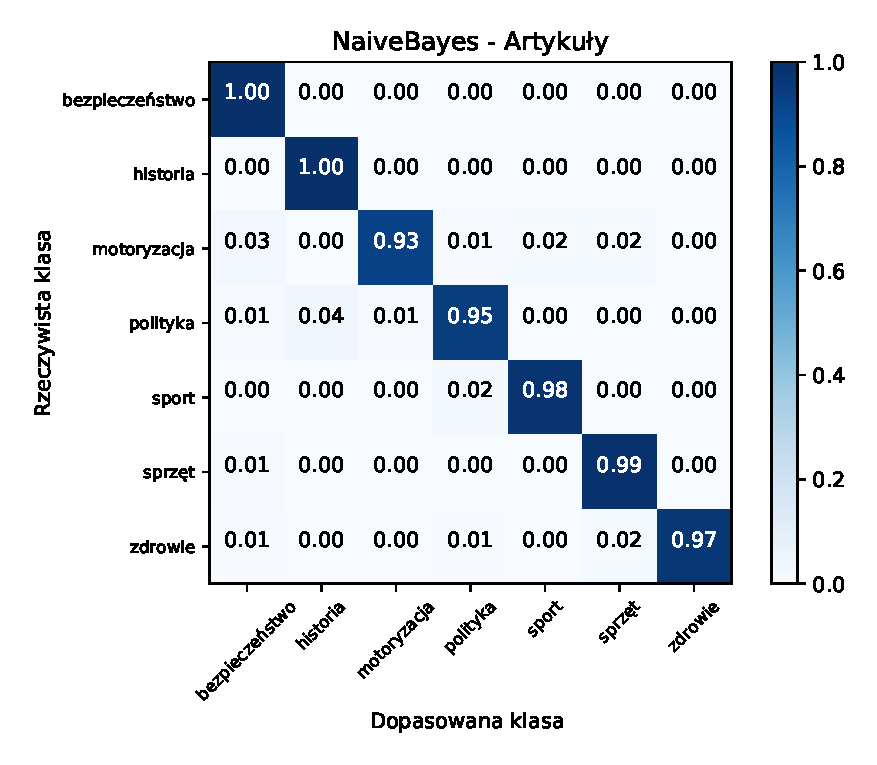
\includegraphics[width=0.45\linewidth]{img/c-matrix-naivebayes-articles}}}
    \qquad
    \subfloat[Artykuły (rzeczowniki)]{{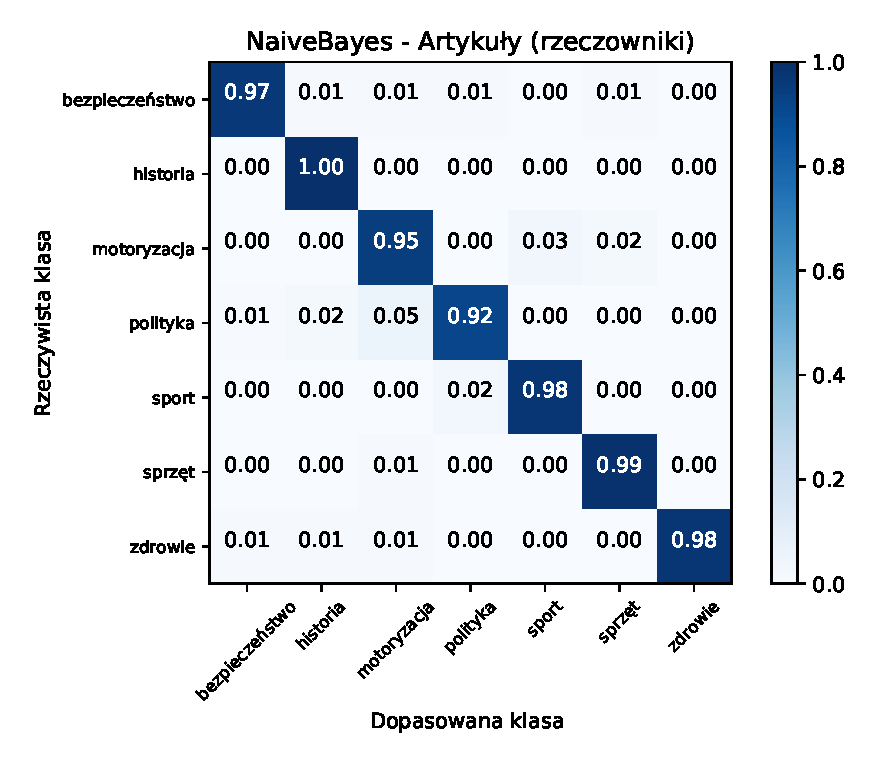
\includegraphics[width=0.45\linewidth]{img/c-matrix-naivebayes-articles-nouns}}}
	\caption{Tablica pomyłek - Drzewo decyzyjne - Artykuły}
    \label{fig:c-matrix-naivebayes-articles}
\end{figure}

W przypadku zbioru z mniejszą liczbą kategorii zaprezentowanych na rysunku \ref{fig:c-matrix-naivebayes-articles} nie zaobserwowano podobnych tendencji. Macierz błędu prezentowała się wzorcowo.

%%%%%%%%%%%%%%%%%%%%%%%%%%%%%%%%%%%%%%%%%%%%%%%%%%%%%%%%%%%%%%%%%%%%%%%%%%%%%%%%%%%%%%%%%%%%%%%%%%%%

\subsection{Dokładność klasyfikacji}
Z analizy wynika, że w każdym z czterech przetestowanych przypadków najszybciej uczącym się klasyfikatorem był \textit{SVM}, natomiast najwolniej uczyło się drzewo decyzyjne; wyniki dla zmodyfikowanej wersji \textit{fastText} są zbliżone do wyników modelu \textit{Bag-Of-Words}. \cite{comparing-svm-and-nb} \cite{walkowiak2018}
\begin{figure}[ht!]
	\centering
	\subfloat[Artykuły]{{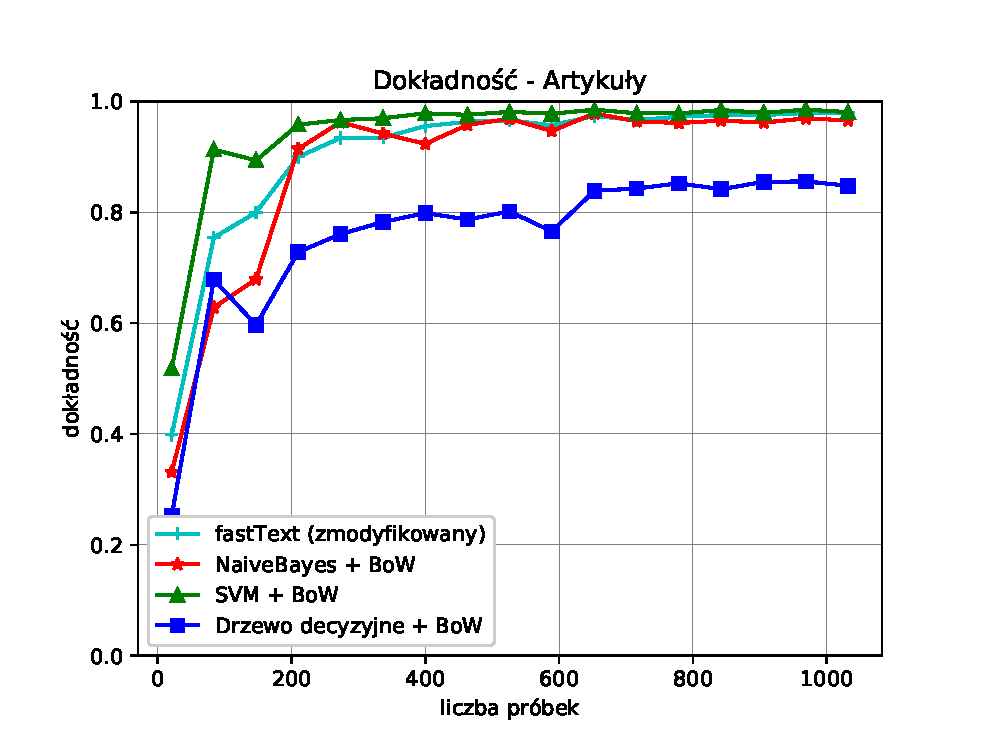
\includegraphics[width=0.45\linewidth]{img/accuracy-articles}}}
    \qquad
    \subfloat[Artykuły (rzeczowniki)]{{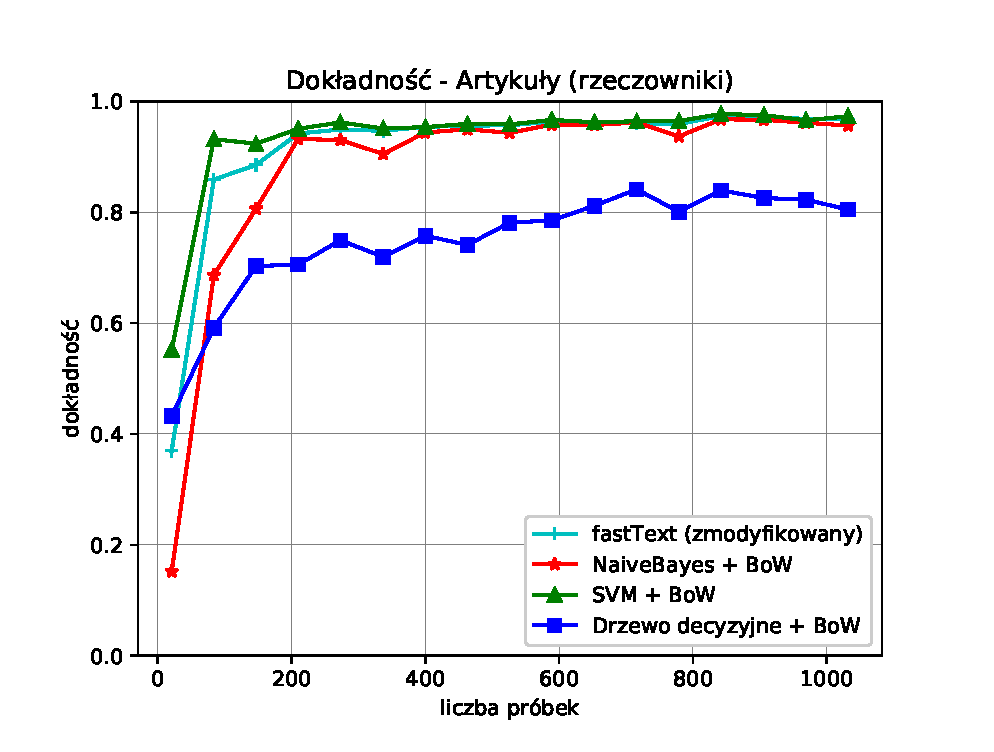
\includegraphics[width=0.45\linewidth]{img/accuracy-articles-nouns}}}
	\caption{Krzywe nauczania Bag-Of-Words oraz fastText - Artykuły}
    \label{fig:learning-curve-articles}
\end{figure}
Dla zbioru z 7 klasami z rysunku \ref{fig:learning-curve-articles} można wywnioskować, iż klasyfikator \textit{SVM} potrzebował zaledwie 14 artykułów z każdej kategorii, aby móc im przyporządkować grupę tematyczną z prawdopodobieństwem na poziomie 93\% dla pełnego korpusu (a) oraz 84\% dla ograniczonego korpusu (b). Odrzucenie słów z innych klas gramatycznych niż rzeczowniki poprawiło szybkość nauczania się klasyfikatora \textit{fastText}, wynik był zbliżony do tego, który był osiągany przez \textit{SVM} w obu przypadkach.  
\begin{figure}[ht!]
	\centering
	\subfloat[Wikipedia]{{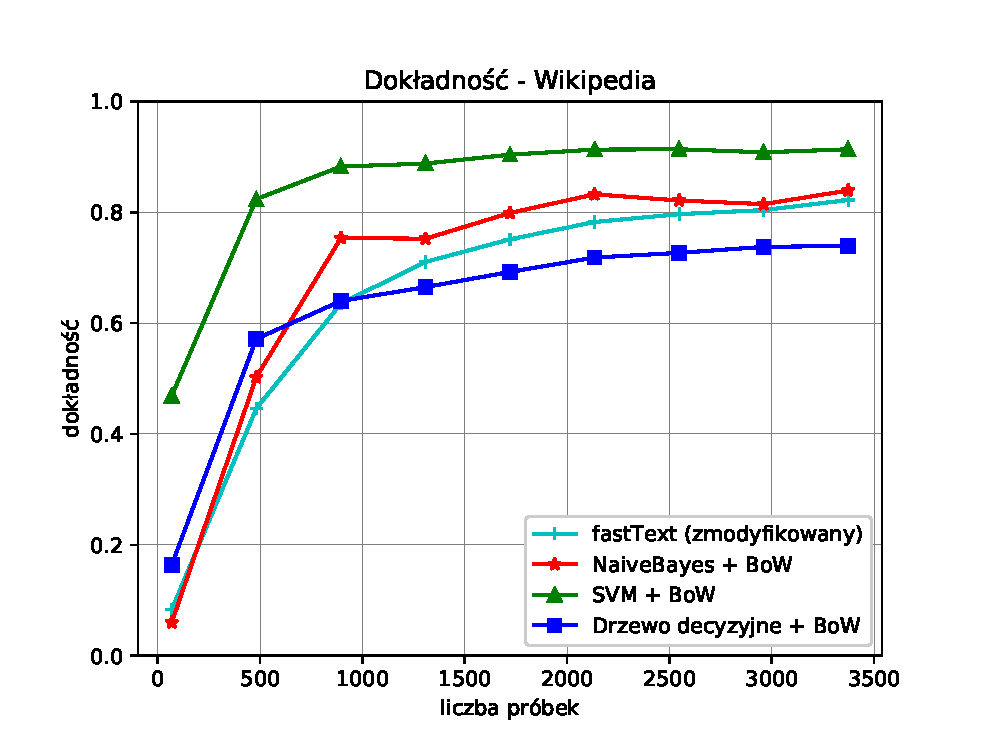
\includegraphics[width=0.45\linewidth]{img/accuracy-wikipedia}}}
    \qquad
    \subfloat[Wikipedia (rzeczowniki)]{{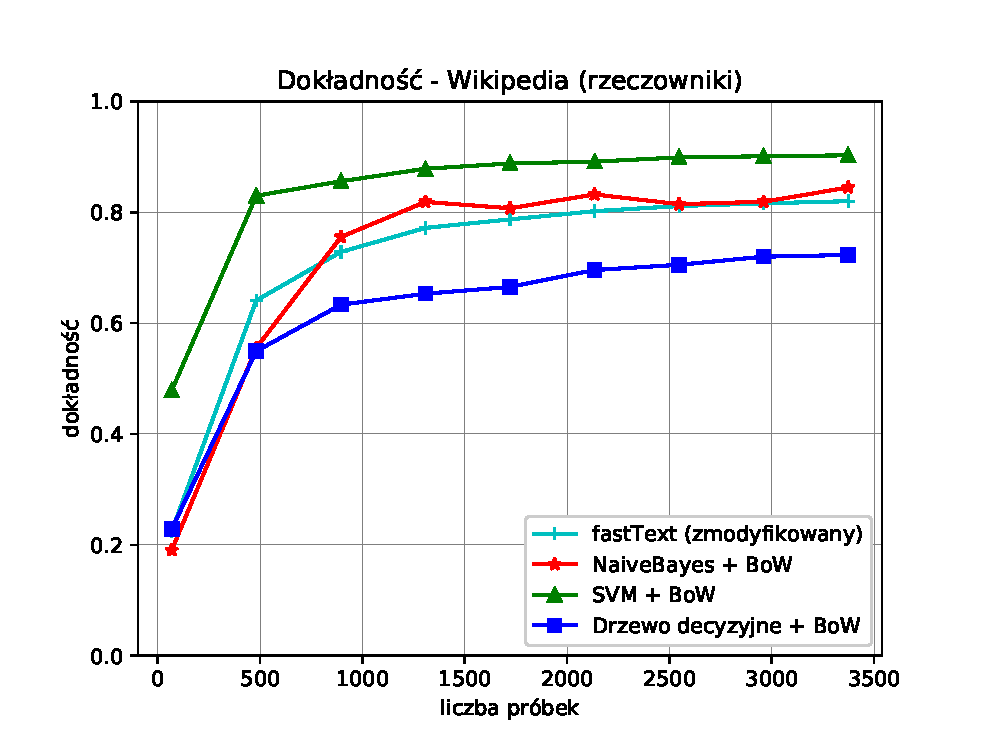
\includegraphics[width=0.45\linewidth]{img/accuracy-wikipedia-nouns}}}
	\caption{Krzywe nauczania Bag-Of-Words oraz fastText - Wikipedia}
    \label{fig:learning-curve-wikipedia}
\end{figure}

Klasyfikatory w przypadku większego zbioru, potrzebowały więcej próbek testowych, aby klasyfikować teksty z wysoką skutecznością, co zostało zobrazowane na wykresach na rysunku \ref{fig:learning-curve-wikipedia}. Wnioski wyciągnięte na podstawie mniejszego zbioru z rysunku \ref{fig:learning-curve-articles} są prawdziwe również w tym przypadku. Ponownie \textit{SVM} uczył się najszybciej, wyniki są odpowiednio niższe, ale tendencja wzrostu jakości została zachowana. Po odrzuceniu innych słów niż rzeczowniki swoje wyniki ponownie polepszył \textit{fastText}, który w pierwszym przypadku dla pełnego zbioru osiągał rezultaty niższe niż \textit{NaiveBayes}, natomiast w drugim przypadku, dla małej liczby próbek zwracał lepsze wyniki. Modyfikacja metody \textit{fastText} postaci odrzucenia innych części mowy niż rzeczowniki nie wpłynęła znacząco na jakość zwracanych wyników. 

%%%%%%%%%%%%%%%%%%%%%%%%%%%%%%%%%%%%%%%%%%%%%%%%%%%%%%%%%%%%%%%%%%%%%%%%%%%%%%%%%%%%%%%%%%%%%%%%%%%%


\subsection{Czas}
Miary jakościowe to nie jedyne istotne wskaźniki; jako że w pracy wykorzystano dwa różne modele, wzięto pod uwagę również czas. Testy czasowe zostały wykonane za każdym razem na tym samym komputerze, wszystkie działające procesy w tle zostały wyłączone na czas testów. Wykorzystany komputer miał specyfikację: 2.2 GHz Intel Core i7, 16 GB 1600 MHz DDR3. Podczas testu stale monitorowano użycie pamięci RAM, w żadnym momencie nie odnotowano jej przekroczenia ani też skokowego spadku, co może wskazywać na to, że aplikacja testująca nie musiała przerywać pracy, aby zapewnić więcej miejsca w pamięci. Pomiędzy testami komputer był uruchamiany ponownie, aby mieć pewność, że warunki testowe za każdym razem będą identyczne. Czas został uśredniony po 10 przebiegach, aby zapobiec przepełnieniu się pamięci podczas badań, co mogłoby skutkować zakłamanymi wynikami.

\newpage
\begin{figure}[ht!]
	\centering
	\subfloat[Artykuły]{{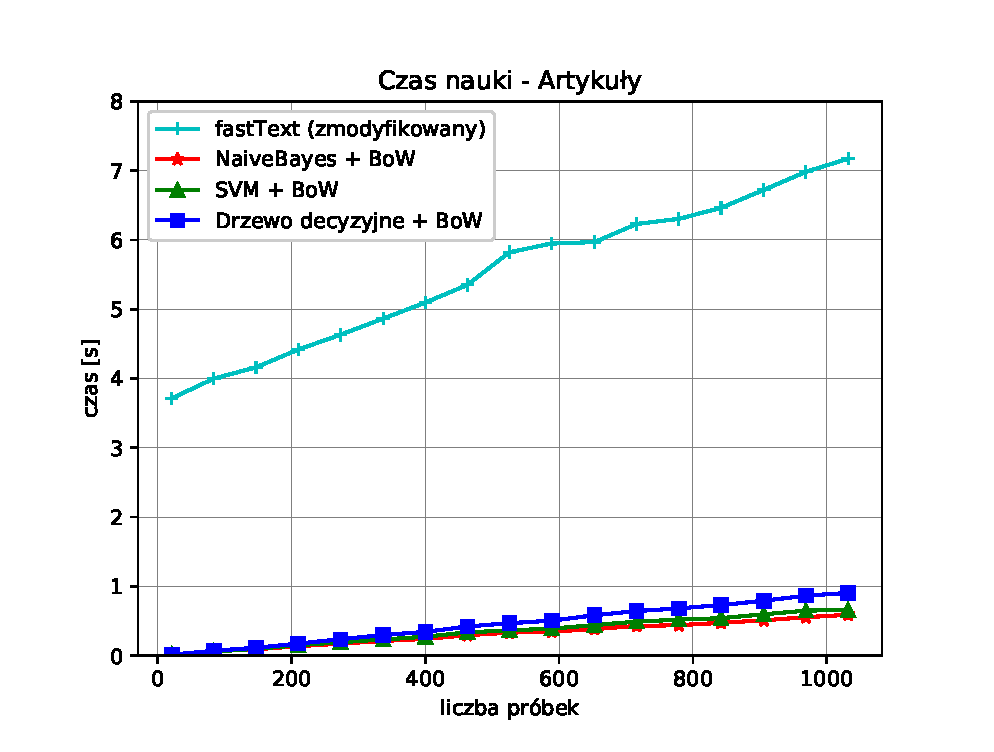
\includegraphics[width=0.45\linewidth]{img/fit-time-articles}}}
    \qquad
    \subfloat[Artykuły (rzeczowniki)]{{\includegraphics[width=0.45\linewidth]{img/fit-time-articles-nouns}}}
	\caption{Porównanie czasu nauki - Artykuły}
    \label{fig:fit-time-articles}
\end{figure}

\begin{figure}[ht!]
	\centering
	\subfloat[Wikipedia]{{\includegraphics[width=0.45\linewidth]{img/fit-time-wikipedia}}}
    \qquad
    \subfloat[Wikipedia (rzeczowniki)]{{\includegraphics[width=0.45\linewidth]{img/fit-time-wikipedia-nouns}}}
	\caption{Porównanie czasu nauki - Wikipedia}
    \label{fig:fit-time-wikipedia}
\end{figure}

Z rysunków \ref{fig:fit-time-articles} oraz \ref{fig:fit-time-wikipedia} wynika, że czas nauki modelu  był ponad 4 razy większy w przypadku narzędzia \textit{fastText} niż \textit{Bag-Of-Words}. Dodatkowo przewaga modelu \textit{BoW} rosła wraz z zwiększającą się liczbą próbek treningowych. 


\begin{figure}[ht!]
	\centering
	\subfloat[Artykuły]{{\includegraphics[width=0.45\linewidth]{img/predict-time-articles}}}
    \qquad
    \subfloat[Artykuły (rzeczowniki)]{{\includegraphics[width=0.45\linewidth]{img/predict-time-articles-nouns}}}
	\caption{Porównanie czasu klasyfikacji - Artykuły}
    \label{fig:predict-time-articles}
\end{figure}

\begin{figure}[ht!]
	\centering
	\subfloat[Wikipedia]{{\includegraphics[width=0.45\linewidth]{img/predict-time-wikipedia}}}
    \qquad
    \subfloat[Wikipedia (rzeczowniki)]{{\includegraphics[width=0.45\linewidth]{img/predict-time-wikipedia-nouns}}}
	\caption{Porównanie czasu klasyfikacji - Wikipedia}
    \label{fig:predict-time-wikipedia}
\end{figure}

Krótki czas potrzebny na sklasyfikowanie dużej ilości dokumentów, zobrazowany na rysunkach \ref{fig:predict-time-articles} oraz \ref{fig:predict-time-wikipedia}, jest niewątpliwą zaletą biblioteki \textit{fastText}. W dużych systemach klasyfikacja jest procesem który  ma kluczowe znaczenie z biznesowego punktu widzenia, ponieważ dane muszą być przetwarzane w czasie rzeczywistym \cite{faster-better-fasttext}. 


\begin{figure}[ht!]
	\centering
	\subfloat[Artykuły]{{\includegraphics[width=0.45\linewidth]{img/total-work-time-articles}}}
    \qquad
    \subfloat[Artykuły (rzeczowniki)]{{\includegraphics[width=0.45\linewidth]{img/total-work-time-articles-nouns}}}
	\caption{Porównanie czasu całkowitej pracy - Artykuły}
    \label{fig:total-time-articles}
\end{figure}

\begin{figure}[ht!]
	\centering
	\subfloat[Wikipedia]{{\includegraphics[width=0.45\linewidth]{img/total-work-time-wikipedia}}}
    \qquad
    \subfloat[Wikipedia (rzeczowniki)]{{\includegraphics[width=0.45\linewidth]{img/total-work-time-wikipedia-nouns}}}
	\caption{Porównanie czasu całkowitej pracy - Wikipedia}
    \label{fig:total-time-wikipedia}
\end{figure}

Dla porównania, całkowity czas pracy obu modeli również wypada na niekorzyść biblioteki \textit{fastText} mimo jej krótkiego czasu klasyfikacji i próby modyfikacji. Wyniki zaprezentowane na rysunkach \ref{fig:total-time-articles} oraz \ref{fig:total-time-wikipedia} są częściowo sprzeczne z oczekiwanymi wynikami \cite{joulin2016bag}. Jedynie czas klasyfikacji \textit{fastText} spełnił oczekiwania i był kilka rzędów mniejszy niż w przypadku drugiego modelu. Długi czas nauki klasyfikatora można wyjaśnić nieoptymalną implementacją wrappera z biblioteki \textit{ShallowLearn}. Dodatkowa implementacja konwertująca dane wejściowe i wyjściowe nie jest przyczyną wyższego czasu nauki, ponieważ liczony jest czas wywoływania jedynie metody rozpoczynającej naukę \textit{fastText}. Drugą możliwą przyczyną, bardziej prawdopodobną, jest zbyt wysoka wartość parametru \textit{epoch}, jednak zmniejszenie tej wartości skutkowałoby zmniejszeniem skuteczności. W przypadku modyfikacji \textit{fastText} zaobserwowano oczekiwany spadek potrzebnego czasu na klasyfikację oraz naukę.
\newpage
\section{Wnioski}
Wyniki przeprowadzonych badań i wyciągnięte wnioski dla zastosowanych metod na dwóch skrajnie różnych korpusach danych, nie stwierdzają wyższości jednej metody czy klasyfikatora ponad resztę. Nie ma oczywistego wyboru jeśli chodzi o najlepszą metodę klasyfikacji tekstu, ponieważ dla każdego systemu istnieją inne istotne współczynnikami, które powinny być brane pod uwagę. W przypadku wyznaczania kategorii dla bardzo dużych zbiorów danych w których czas ma kluczowe znaczenie, np. Facebook lub inne systemy informatyczne, oczywistym wyborem będzie \textit{fastText} ze względu na bardzo krótki czas wykonania i odpowiedzi na dane wejściowe w przypadku klasyfikacji. Czas nauki w tym przypadku odgrywa znacznie mniejszą rolę, ponieważ raz nauczony model będzie w stanie klasyfikować dokumenty na wystarczająco dobrym poziomie. Nauka klasyfikatora w przypadku dużych rozproszonych systemów odbywać się będzie asynchronicznie, co dodatkowo umniejsza istotność czasu nauczania. W przypadku, gdy system nastawiony jest na zwracanie jak najbardziej poprawnych wyników, gdzie różnica czasowa rzędu kilku godzin nie ma aż tak dużego wpływu, zdecydowanie lepszym wyborem będzie zastosowanie klasycznego modelu \textit{Bag-Of-Words}. Warto również pamiętać, że olbrzymi wpływ na wybór metody lub klasyfikatora powinna mieć perspektywa ilości danych, które zostaną użyte w systemie. To właśnie liczebność zbiorów jest główną sfer, która powinna być brana pod uwagę przy wyborze. W przypadku modelu \textit{Bag-Of-Words} klasyfikator \textit{SVM} radził sobie najlepiej, należy jednak pamiętać, że nie jest to reguła która będzie się powtarzać dla każdego zbioru danych. Na uwagę zasługuje również fakt, że ograniczenie zbioru do samych rzeczowników wyraźnie zmniejszyło czas potrzebny na predykcję oraz naukę zastosowanych klasyfikatorów. Korpusy zawierające same rzeczowniki zmniejszyły swoją objętość wagową od 20 do 30\% co stanowi prawie 1/3 całości danych; mimo tak dużego ubytku danych jakość średniej klasyfikacji pogorszyła się minimalnie, a na podstawie przebadanych miar różnica wynosiła nie więcej niż 2\% dla miary f1. Co więcej, w niektórych przypadkach usunięcie słów innych niż rzeczowniki pozytywnie wpłynęło na jakość znajdowanych klas; dotyczy to głównie słabo rozpoznawanych kategorii, choć nie jest to regułą, ale można zauważyć pewną powtarzalność.